%\VignetteIndexEntry{distr - manual}
%\VignetteDepends{startupmsg,distr}
%\VignetteKeywords{probability distribution,simulation,estimation}
%\VignettePackage{distr}
%
\documentclass[11pt]{article}
\usepackage{geometry}\usepackage{color}
\usepackage{ifpdf}
\definecolor{darkblue}{rgb}{0.0,0.0,0.75}
\usepackage{amssymb}
\usepackage[%
baseurl={http://www.bioconductor.org},%
pdftitle={S4 Classes for Distributions---a manual for packages distr, distrSim, distrTEst, and distrEx},%
pdfauthor={Peter Ruckdeschel, Matthias Kohl, Thomas Stabla, Florian Camphausen},%
pdfsubject={distr},%
pdfkeywords={probability distribution,simulation,estimation},%
pagebackref,bookmarks,colorlinks,linkcolor=darkblue,citecolor=darkblue,%
pagecolor=darkblue,raiselinks,plainpages,pdftex]{hyperref}
%
\markboth{\sl Packages ``{\tt distr}'', ``{\tt distrSim}'', ``{\tt distrTEst}'', 
``{\tt distrEx}'', ``{\tt distrTeach}''}%
{\sl Packages ``{\tt distr}'', ``{\tt distrSim}'', ``{\tt distrTEst}'',  
``{\tt distrEx}'', ``{\tt distrTeach}''}
%
% -------------------------------------------------------------------------------
\newcommand{\code}[1]{{\tt #1}}
\newcommand{\pkg}[1]{{\tt "#1"}}
\newcommand{\pkgversion}{{\tt 2.0}}
\newcommand{\pkgExversion}{{\tt 2.0}}
\newcommand{\Reals}{\mathbb{R}}
\newcommand{\R}{\mathbb{R}}
\newcommand{\N}{\mathbb{N}}
% -------------------------------------------------------------------------------
% new from version 2.5 of R:
% -------------------------------------------------------------------------------

% -------------------------------------------------------------------------------
%
% -------------------------------------------------------------------------------
\usepackage{/home/btm722/RTOP/r-devel/R/share/texmf/Sweave}
\begin{document}
% -------------------------------------------------------------------------------
\title{{\tt S4} Classes for Distributions---a manual for packages \pkg{distr}, 
        \pkg{distrEx}, \pkg{distrSim}, \pkg{distrTEst}, \pkg{distrTeach}, 
        version \pkgversion}
%,version \pkgExversion}
\author{\small Peter Ruckdeschel\thanks{Universit\"at Bayreuth}
\\[-.5ex]
\small Matthias Kohl\thanks{SIRS-Lab GmbH, Jena}
\\[-.5ex]
\small Thomas Stabla\thanks{Hans-Sachs-Gymnasium N\"urnberg}
\\[-.5ex]
\small Florian Camphausen\thanks{West-LB, D\"usseldorf}
\smallskip\\
\small Mathematisches Institut\\[-.5ex]
\small Universit\"at Bayreuth\\[-.5ex]
\small D-95440 Bayreuth\\[-.5ex]
\small Germany\\
\small e-Mail: {\small \tt peter.ruckdeschel@uni-bayreuth.de}\\
}
\maketitle
% -------------------------------------------------------------------------------
\begin{abstract}
% -------------------------------------------------------------------------------
\pkg{distr} is a package for {\sf R} from version {\tt 1.8.1} onwards that is 
distributed under {\tt GPL} license 2.0. Its own current version is \pkgversion.
%
The aim of this package is to provide a conceptual treatment of random variables 
(r.v.'s) by means of {\tt S4}--classes. A mother class \code{Distribution} is 
introduced with slots for a parameter and for functions {\tt r},  {\tt d}, 
{\tt p}, and {\tt q} for simulation, respectively for evaluation of density / 
c.d.f.\ and quantile function of the corresponding distribution. All 
distributions of the \pkg{stats} package are implemented as subclasses of either 
\code{AbscontDistribution} or \code{DiscreteDistribution},
which themselves are again subclasses of \code{UnivariateDistribution}. %\\
%
By means of these classes, we may automatically generate new objects of these 
classes for the laws of r.v.'s under standard mathematical univariate 
transformations and under convolution of independent r.v.'s.
%
From version 1.6 on, \pkg{distr} has been split up into the smaller packages
\pkg{distr} (only distribution-classes and -methods),  \pkg{distrSim}
(standardized treatment of simulations, also under contaminations)
and \pkg{distrTEst} \newline(classes and methods for evaluations of statistical
procedures on such simulations).

\noindent The latter two of them require package \pkg{setRNG} by 
\href{mailto:pgilbert@bank-banque-canada.ca}{Paul Gilbert}
to be installed from \href{http://cran.r-project.org/mirrors.html}{\tt CRAN}. 
% \\

\noindent Additionally, mainly contributed by \cite{MK:05}, in \pkg{distrEx} we 
extend the functionality of \pkg{distr}, providing functionals like expectation 
or variance and distances for distributions. Also, this package contains some 
first steps to multivariate distributions, providing classes for discrete 
multivariate distributions and for factorized, conditional
distributions.
% -------------------------------------------------------------------------------
\end{abstract}
% -------------------------------------------------------------------------------
\tableofcontents
\noindent
{\small This document appeared in an abridged form in {\em R-News\/}, {\bf 6}(2) 
as {\sf ``S4 Classes for Distributions''}, c.f.\ \cite{R:K:S:C:04}, which in its 
published form refers to package versions 1.6, resp.\ 0.4-2. This document takes 
into account the subsequent revisions and versions.}\medskip
% -------------------------------------------------------------------------------
\addtocounter{section}{-1}
\section{Motivation}
% -------------------------------------------------------------------------------
{\sf R} up to now contains powerful techniques for virtually
any useful distribution using the suggestive naming convention
{\tt [prefix]<name>} as functions where {\tt [prefix]} stands for
 {\tt r}, {\tt d}, {\tt p}, or {\tt q}
 and {\tt <name>} is the name of the distribution.\\
There are limitations of this concept, however:
You can only use distributions which are implemented in some library
already or for which you yourself have provided an implementation.
In many natural settings you want to formulate algorithms once for
all distributions, so you should be able to treat the actual distribution 
{\tt <name>} as sort of a variable.\\
You may of course paste together prefix and the value of {\tt <name>} as a 
string and then use \code{eval(parse(....))}. This is neither very elegant nor 
flexible, however.\\
%
Instead, we would rather like to implement the algorithm by passing an object of 
some distribution class as argument to the function. Even better though, we 
would use a generic function and let the {\tt S4}-dispatching mechanism decide 
what to do at run-time. In particular, we would like to automatically generate 
the corresponding functions {\tt r}, {\tt d}, {\tt p}, and {\tt q} for the law 
of expressions like \code{X+3Y} for objects \code{X} and \code{Y} of class 
\code{Distribution}, or, more general, of a transformation of $X$, $Y$ under a 
function $f\colon \Reals^2 \to \Reals$ which is already realized as a function 
in {\sf R}.\\
This is possible with package \pkg{distr}. As an example, try
\begin{Schunk}
\begin{Sinput}
> library(distr)
> N <- Norm(mean = 2, sd = 1.3)
> P <- Pois(lambda = 1.2)
> Z <- 2*N + 3 + P
> Z
\end{Sinput}
\begin{Soutput}
Distribution Object of Class: AbscontDistribution
\end{Soutput}
\begin{Sinput}
> plot(Z, withSweave = TRUE)
> p(Z)(0.4)
\end{Sinput}
\begin{Soutput}
[1] 0.002404514
\end{Soutput}
\begin{Sinput}
> q(Z)(0.3)
\end{Sinput}
\begin{Soutput}
[1] 6.709
\end{Soutput}
\begin{Sinput}
> Zs <- r(Z)(50)
> Zs
\end{Sinput}
\begin{Soutput}
 [1] 15.226388  7.564565  9.305538  3.656730  7.501088  8.949388  7.270903
 [8]  8.590010  8.234551  8.027369  7.755364  6.475394  2.453460  8.461635
[15]  6.344245  4.269209  9.750363  7.230705  2.033280  2.883308  5.015167
[22]  9.241034  2.496826  7.757291  8.241218  6.861682  8.066679  6.566020
[29] 14.076574  3.960959  7.774985 10.029283  9.905783  5.414182  7.356253
[36]  9.795385  5.912620  7.338719  6.764604 12.652007 11.374727  5.701335
[43]  4.971393  7.244023 10.766473 10.886731  6.591946  7.642596  6.791444
[50]  8.511914
\end{Soutput}
\end{Schunk}
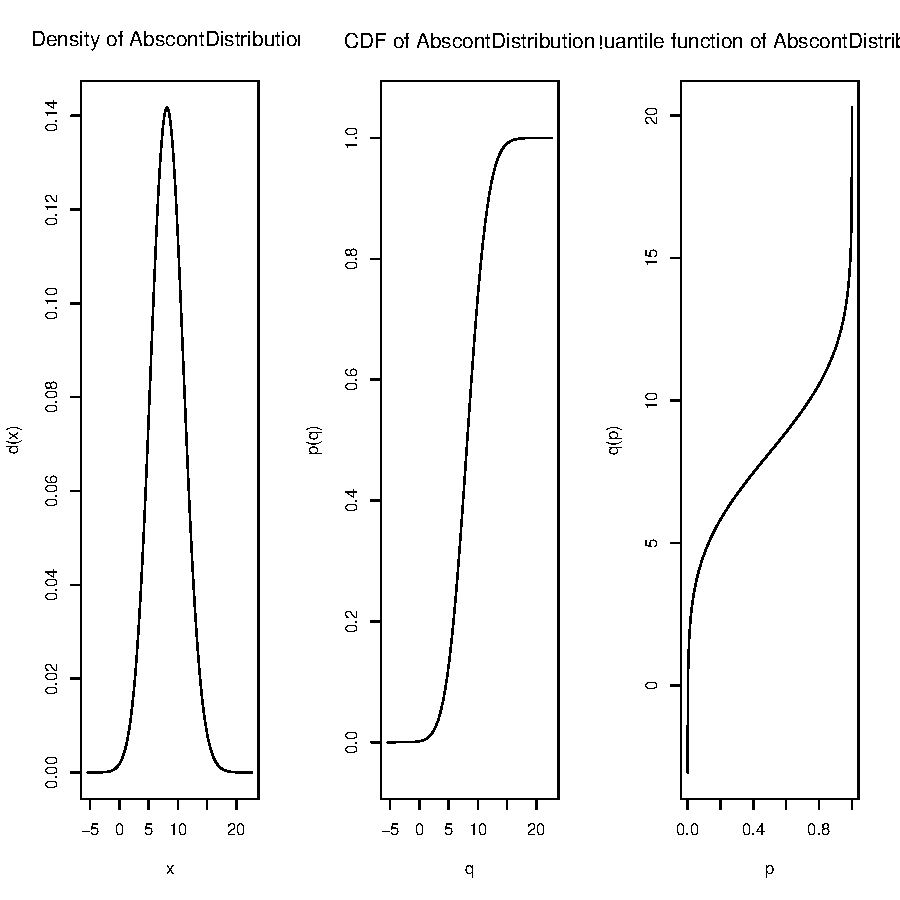
\includegraphics{distr-exam1}
\par
\begin{small}
\noindent{\bf Comment:}\\
Let \code{N} an object of class \code{"Norm"} with parameters  \code{mean=2},
\code{sd=1.3} and let \code{P}  an object of class \code{"Pois"} with parameter 
\code{lambda=1.2}. Assigning to \code{Z} the expression \code{2*N+3+P}, a 
new distribution object is generated ---of class \code{"AbscontDistribution"} in 
our case--- so that identifying \code{N}, \code{P}, \code{Z} with random 
variables distributed according to {\tt N}, {\tt P}, {\tt Z}, 
${\cal L}({\tt Z})={\cal L}(2*{\tt N}+3+{\tt P})$,  and writing \code{p(Z)(0.4)}  
we get $P(Z\leq 0.4)$, \code{ q(Z)(0.3)}  the $30\%$-quantile of {\tt Z},
and with \code{r(Z)(50)} we generate $50$ pseudo random numbers distributed 
according to {\tt Z}, while the \code{plot} command generates the above figure.
\end{small}
% -------------------------------------------------------------------------------
\section{Concept}
% -------------------------------------------------------------------------------
In developing our packages, we had the following principles in mind:
We wanted to be open in our design so that our classes could easily be extended 
by any volunteer in the {\sf R} community to provide more complex classes of 
distributions as multivariate distributions, times series distributions, 
conditional distributions. As an exercise, the reader is encouraged to implement 
extrem value  distributions from the package \pkg{evd}\footnote{a solution to 
this ``homework''  may be found in the sources to \pkg{distrEx}}. The largest 
effort will in fact be the documentation\ldots\\
We also wanted to preserve naming and notation from {\sf R}-\pkg{stats}
as far as possible so that any programmer used to {\tt S} could quickly
use our package. Even more so, as the distributions already implemented to
{\sf R} are all well tested and programmed with skills we lack, we use the
existing {\tt r}, {\tt d}, {\tt p}, and {\tt q}-functions wherever possible,
only wrapping them by small code sniplets to our class hierarchy.\\
Third we wanted to use a suggestive notation for our automatically generated
methods \code{r}, \code{d}, \code{p}, and \code{q}, which we think is now 
largely achieved. All this should make intensive use of object orientation in 
order to be able to use inheritance and method overloading.
Let us briefly explain why we decided to realize \code{r}, \code{d},
\code{p}, and \code{q} as part of our class definitions:
Doing so, we place ourselves somewhere between
pure object orientation where methods would be {\it slots\/} ---in the language 
of the {\tt S4}-concept, confer \cite{Cham:98}--- and the {\tt S4} paradigm 
where methods ``live their own life'' apart from the classes, or, to \code{q}, 
which should be regarded use \cite{Beng:03}'s terminology, we use 
COOP\footnote{class-object-orientated 
programming, as e.g.\ in {\tt C++}}-style for \code{r}, \code{d}, \code{p}, and 
\code{q} methods, and FOOP\footnote{function-object-orientated programming, 
as in the {\tt S4}-concept} -style for "normal" methods.\\
The {\tt S4}-paradigm with methods which are not attached to an object but 
rather behave differently according to the classes of their arguments is fine 
if there are particular user-written methods for only some few general 
distribution classes like  \code{AbscontDistribution}, as in the case for 
\code{plot} or \code{"+"} (c.f.\ \cite{K:R:S:04}, Section 2.2). 
During a typical {\sf R} session with \pkg{distr}, however, there will be a lot 
of, mostly automatically generated objects of our distribution classes, each 
with its own \code{r}, \code{d}, \code{p}, and \code{q}; this even applies to 
intermediate expressions like \code{2*N}, \code{2*N+3} to eventually produce 
\code{Z} in the example in the motivation. Treating \code{r}, \code{d}, 
\code{p}, and \code{q} as generic functions, we would need to generate new 
classes for each expression \code{2*N}, \code{2*N+3}, \code{Z} and, 
correspondingly, particular {\tt S4}-methods for \code{r}, \code{d}, \code{p}, 
and \code{q} for each of these new classes; apparently, this would produce 
overly many classes for an effective inheritance structure. \\
In providing arithmetics for distributions, we have to deviate a little from
the paradigm of {\tt S} as a functional language: For operators like ``$+$'',
additional parameters controlling the precision of the results cannot be handily
passed as arguments. For this purpose we provide global options which may be
inspected and modified by \code{distroptions}, 
\code{getdistrOption}\footnote{Upto version 0.4-4, we used a different mechanism 
to inspect/modify global options of \pkg{distrEx} (see 
section~\ref{distrExoptions}); corresponding functions \code{distrExoptions}, 
\code{getdistrExOption} for package \pkg{distrEx} are available from version 
1.9 on.} in complete analogy to \code{options}, \code{getOption}.
%
Finally our concept as to parameters: Contrary to the standard {\sf R}-functions 
like \code{rnorm} we only permit length $1$ for parameters like \code{mean}, 
because we see the objects as implementations of univariate random variables, 
for which vector-valued parameters make no sense; rather one could gather 
several objects with possibly different parameters to a vector/list of 
distributions. Of course, the original functions \code{rnorm} etc.\ remain 
unchanged and still allow for vector-valued parameters.
Kouros Owzar  in an off-list mail raised the point, that in case of multiple 
parameters as in case of the normal or the $\Gamma$-distribution, it might be 
useful to be able to pass these multiple parameters in vectorized form to the 
generating function. We, too, think that this is a good idea, but even more plan 
to introduce a further extension package to \pkg{distr} which will cover 
statistical models. In this package, this issue will be solved by requiring a 
map $\theta \mapsto P_\theta$ or, in {\tt S}, a function 
\code{function(theta){....}} which returns an object of class distribution 
or subclass, which realizes $P_\theta$. So it will be up to the programmer or 
user how to realize this map.
% -------------------------------------------------------------------------------
\section{Organization in classes}
% -------------------------------------------------------------------------------
Loosely speaking we have three large groups of classes: distribution classes (in 
\pkg{distr}), simulation classes (in \pkg{distrSim}) and an evaluation class (in 
\pkg{distrTEst}), where the latter two are to be considered only as tools which 
allow a unified treatment of simulations and evaluation of statistical estimation 
(perhaps also tests and predictions later) under varying simulation situations.
Additionally, package \pkg{distrEx} provides classes for discrete multivariate 
distributions and for factorized, conditional distributions, as well as a bundle 
of functionals and distances (see below).
% -------------------------------------------------------------------------------
\subsection{Distribution classes}
% -------------------------------------------------------------------------------
The purpose of the classes derived from the class \code{Distribution}  is to 
implement the concept of a r.v./distribution as such in {\sf R}.\\
All classes derived from \code{Distribution} have a slot \code{param} for a 
parameter, a slot \code{img} for the range and the constitutive slots \code{r}, 
\code{d}, \code{p}, and \code{q}.\\
From version 1.9 on, up to arguments referring to a parameter of the 
distribution (like \code{mean} for the normal distribution), these function 
slots have the same arguments as those of package \pkg{stats}, i.e.; for a 
distribution object \code{X} we may call these functions as 

\begin{itemize}
\item \code{r(X)(n)}  $\qquad$ ---except for objects of class \code{Hyper},
where there is a slot \code{n} already, so here the argument name 
to \code{r} is \code{nn}.
\item \code{d(X)(x, log = FALSE)}
\item \code{p(X)(q, lower.tail = TRUE, log.p = FALSE)}
\item \code{q(X)(p, lower.tail = TRUE, log.p = FALSE)}
\end{itemize}

For the arguments of these function slots see e.g.\ \code{rnorm}
from package \pkg{stats}.
Note that, as usual, slots \code{d}, \code{p}, and \code{q} are vectorized
in their first argument, but are not on the subsequent ones.
The idea is to gain higher precision for the upper tails or when multiplying
probabilities.
% -------------------------------------------------------------------------------
\subsubsection{Subclasses}
% -------------------------------------------------------------------------------
To begin with, we have considered univariate distributions giving the 
{\tt S4}-class \code{UnivariateDistribution}, and as typical subclasses, we 
have introduced classes for absolutely continuous and discrete distributions 
---\code{AbscontDistribution} and \code{DiscreteDistribution}.\\

The former, from version 1.9 on, has a slot \code{gaps} of class 
\code{OptionalMatrix}, i.e.; an object which may either be \code{NULL} or
a \code{matrix}. This slot, if non-\code{NULL}, contains left and right 
endpoints of intervals where the density of the object is $0$. This slot 
may be inspected by the accessor \code{gaps()} and modified by a corresponding
replacement method. It may also be filled automatically by 
\code{setgaps(object, exactq = 6, ngrid = 50000)}, where upon evaluation of 
the \code{d}-slot on a grid of length \code{ngrid}, all regions in the 
range\footnote{more precisely: between lower and upper \code{TruncQuantile};
 \code{TruncQuantile} is a global option of  \pkg{distr} described in 
 section~\ref{options}} of the distribution where the density is smaller than 
 $10^{\scriptscriptstyle - {\rm exactq}}$ are set to gaps.\\ For saved objects 
 from earlier versions, we provide the functions \code{isOldVersion} and 
 \linebreak[4]\code{conv2NewVersion} to check whether the
object was generated by an older version of this package and
to convert such an object to the new format, respectively.\\

Class \code{DiscreteDistribution} has a slot \code{support}, a vector containing 
the support of the distribution, which is truncated to the lower/upper 
\code{TruncQuantile} in case of an infinite support. \code{TruncQuantile} is a 
global option of  \pkg{distr} described in section~{\ref{options}}. 
From version 1.9 on, there are methods \code{p.l} and \code{q.r} for the 
left-continuous variant of the cdf, i.e.; $t\mapsto {\rm p.l}(t)=P(X<t)$), and the 
right-continuous variant of the quantile function, i.e.;
$$
s\mapsto {\rm q.r}(s)=\sup\{t \,\big|\, P({\tt object}\leq t)\leq s\}
$$
Also from version 1.9 on, class \code{DiscreteDistribution} has a subclass 
\code{LatticeDistribution} for supports consisting of\footnote{or at least
if filled with points carrying no mass have a representation as an affine linear 
lattice} an affine linear lattice of form $p+iw$ for $p\in\R$, $w\in\R$, 
$w\not=0$ and $i=0,1,\ldots,L$, 
$L\in\N \cup\infty$. This class gains a slot \code{lattice} of 
class \code{Lattice} (see below). The purpose of this class is mainly its use 
in DFT/FFT methods for convolution. Slot \code{lattice} may be 
inspected by the usual accessor function \code{lattice()}.
As by inheritance, all subclasses of \code{LatticeDistribution} which prior to
version 1.9 were direct subclasses of \code{DiscreteDistribution} gain a 
slot \code{lattice}, too, we provide again \code{isOldVersion} and 
\code{conv2NewVersion} methods to check whether the object was generated by an 
older version of this package and to convert such an object to the new 
format, respectively. Also note that internally, we suppress lattice points from 
the support where the probability is $0$.\\        


Objects of classes \code{LatticeDistribution} resp.\ 
\code{DiscreteDistribution} may be generated using the generating functions
\code{LatticeDistribution()} resp.\ \code{DiscreteDistribution()}; see also
the corresponding help.
\\
As subclasses of these absolutely continuous and discrete classes, we have 
implemented all parametric families which already exist in the  \pkg{stats} 
package of {\sf R} in form of 
{\tt [prefix]<name>} functions ---by just providing wrappers to the original 
{\sf R}-functions.\\
%
Schematically, the inheritance relations as well as the slots 
of  the corresponding classes may be read off from figure~\ref{fig1c}. 
Class \code{LatticeDistribution} and slot \code{gaps}, as well as
additional classes \code{AffLinAbscontDistribution}, 
\code{AffLinDiscreteDistribution}, \code{AffLinLatticeDistribution} 
(c.f.\ section~\ref{afflin}) are still lacking in this graphic so far, however.
\\

\ifpdf
\begin{figure}[!ht]\label{fig1}
\vspace{2ex}
  \begin{center}
%    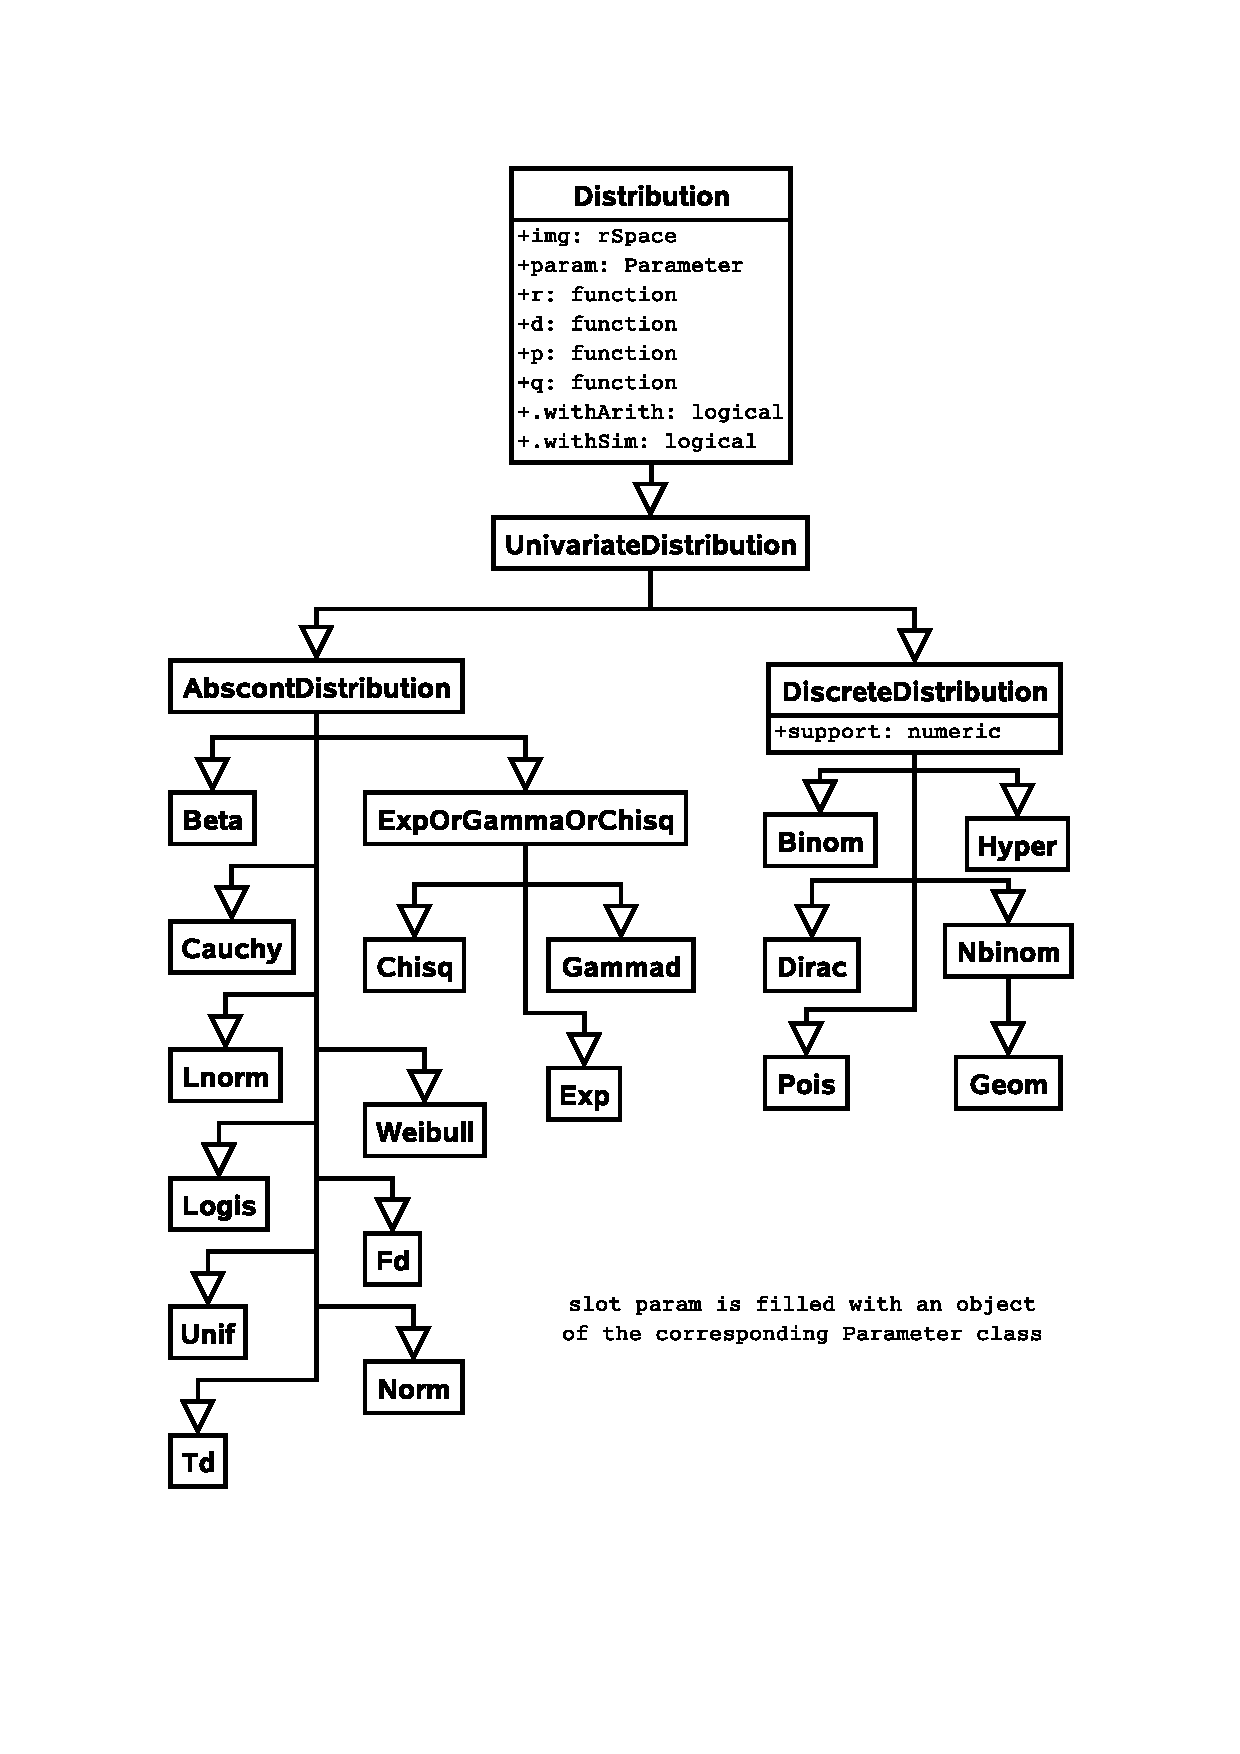
\includegraphics[viewport=0 0 500 700,width=9cm]{distribution.pdf}%
    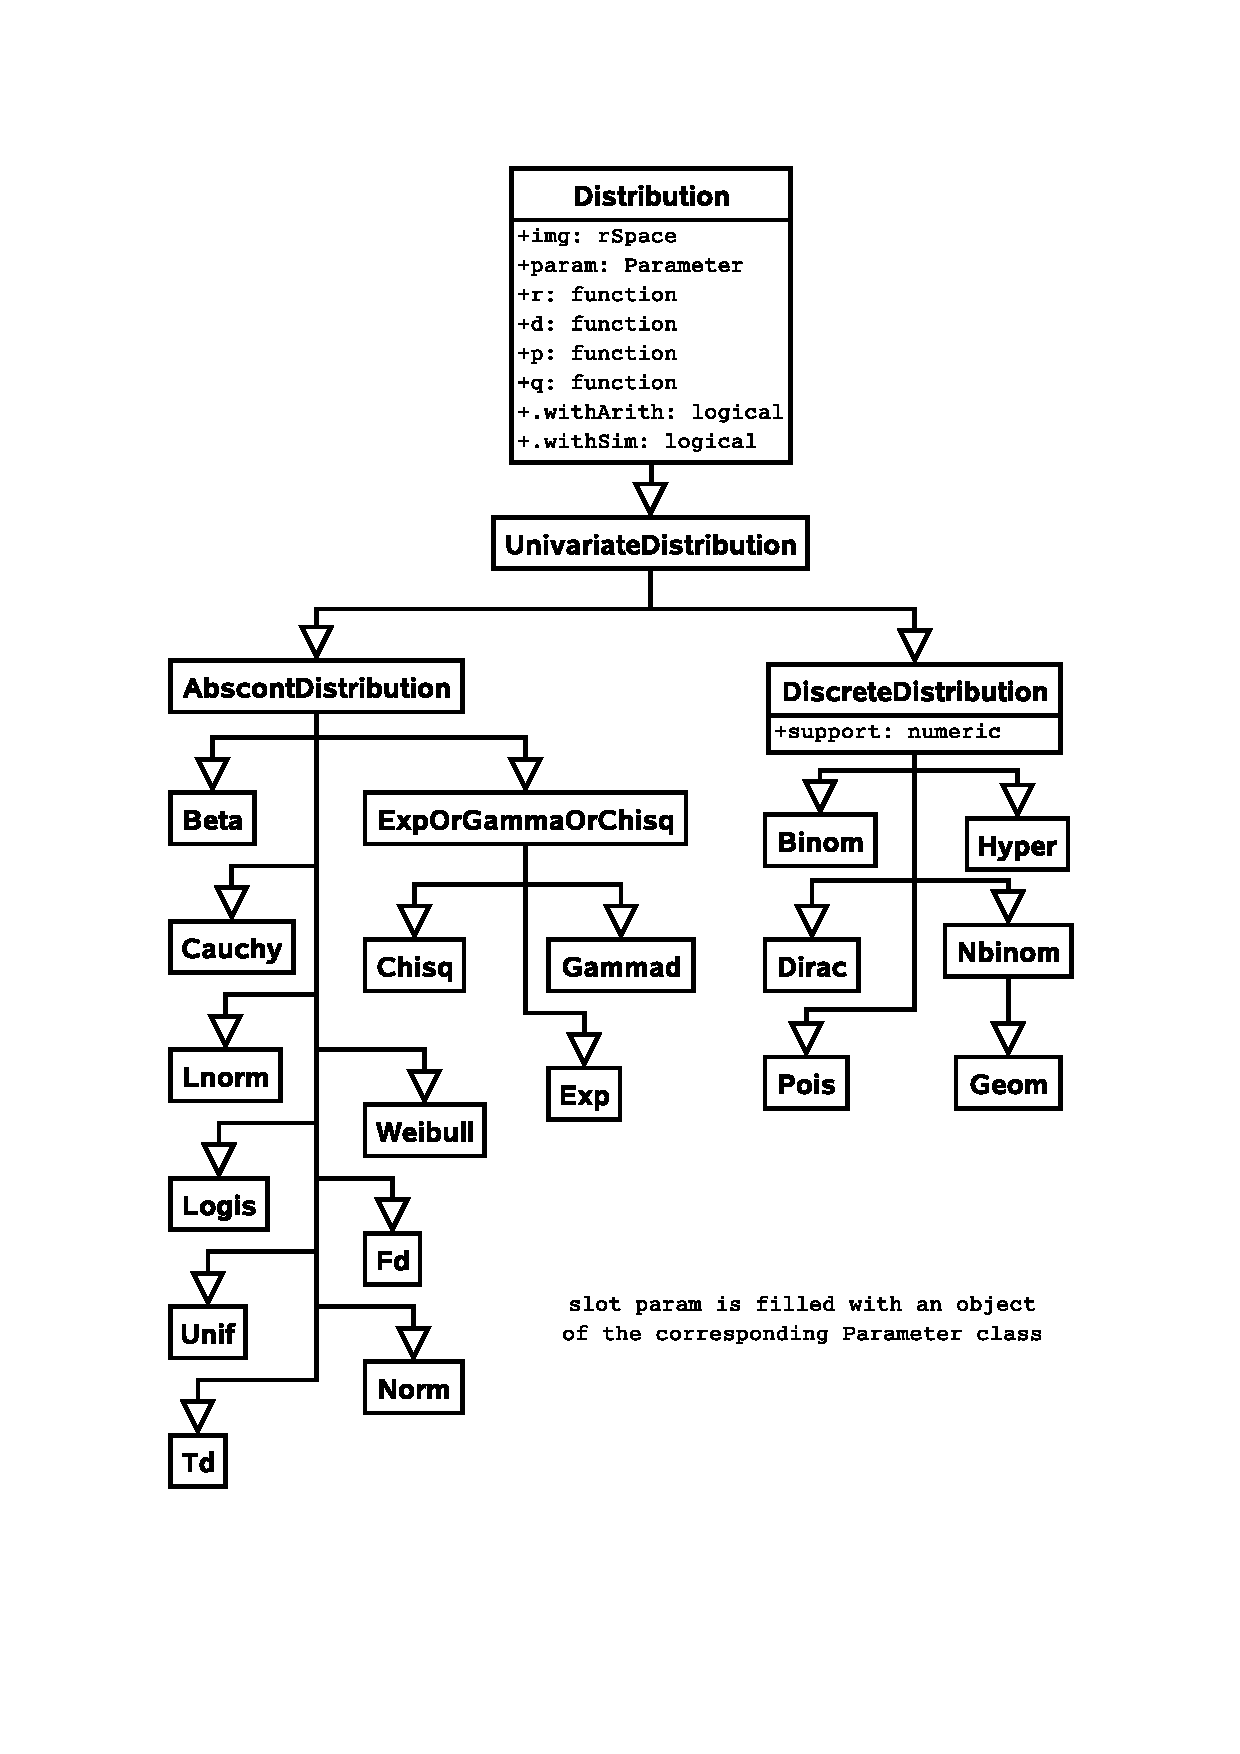
\includegraphics[viewport=130 150 500 750,width=9cm]{distribution.pdf}%
    \caption{\label{fig1c}{\footnotesize Inheritance relations and slots of the 
    corresponding \mbox{(sub-)}classes for \code{Distribution} where we do not
    repeat inherited slots
    }}
  \end{center}
\vspace{-4ex}
\end{figure}
\else
\begin{figure}[htb]\label{fig1}
  \begin{center}
    \includegraphics[viewport=130 150 500 730,width=7.5cm]{distribution.ps}%
    \caption{\label{fig1c}{\footnotesize Inheritance relations and slots of the 
    corresponding \mbox{(sub-)}classes for \code{Distribution} where we do not 
    repeat inherited slots
    }}
  \end{center}
\vspace{-1ex}
\end{figure}
\fi
The most powerful use of our package probably consists in operations to 
automatically generate new slots \code{r}, \code{d}, \code{p}, and \code{q} 
---induced by mathematical transformations. This is discussed in some detail in 
subsection~{\ref{methods}}.
%
\subsubsection{Classes for multivariate distributions and for conditional 
distributions}

In \pkg{distrEx}, we provide the following classes for handling multivariate 
distributions:

\paragraph{Lists of distributions}

As a first step, we allow distributions to be gathered in lists, giving
classes \code{DistrList} and \code{UnivarDistrList}, where in case of the latter,
all elements must be univariate distributions. For these, the usual indexing 
operations with \code{[[.]]} are available. As we will use these lists to 
construct more general mixture distributions in some subsequent versions, we 
have moved these routines to package \pkg{distr} from version 1.9 on.

\paragraph{Multivariate distribution classes}

Multivariate distributions are much more complicated than univariate ones,
which is why but a few exceptional ones have already been implemented to R in
packages like \pkg{multnorm}. In particular it is not so clear what a slot 
\code{q} should mean and, in higher dimensions slot \code{p}, and possibly also 
slot \code{d} may become awkward. So, for multivariate distributions, realized 
as class \code{MultivariateDistribution}, we only insist on slot \code{r}, while 
the other functional slots may be left void.

The easiest case is the case of a discrete multivariate distribution with finite 
support which is implemented as class \code{DiscreteMVDistribution}.

\paragraph{Conditional distribution classes}

Also arising in multivariate settings only are conditional distributions. In our 
approach, we realize factorized, conditional distributions where the 
(factorized) condition is in fact treated as an additional parameter to the 
distribution. The condition is realized as an object of class \code{Condition}, 
which is a slot of corresponding classes \code{UnivariateCondDistribution}. 
This latter is the mother class to classes
\code{AbscontCondDistribution} and \code{DiscreteCondDistribution}.
The most important application of these classes so far is regression, where
the distribution of the observation given the covariates is just realized as
a \code{UnivariateCondDistribution}.

\subsubsection{Parameter classes}
%
As most distributions come with a parameter which often is of own interest, we 
endow the corresponding slots of a distribution class with an own parameter 
class, which allows for some checking like ``Is the parameter \code{lambda} of 
an exponential distribution non-negative?'',
``Is the parameter \code{size} of a binomial a positive integer?''\\
Consequently, we have a method \code{liesIn} that may answer such questions by a 
\code{TRUE}/\code{FALSE} statement. Schematically, the inheritance relations of 
class \code{Parameter} as well as the slots of the corresponding
\mbox{(sub-)}classes may be read off in figure~\ref{fig4c} where we do not 
repeat inherited slots.
%
\ifpdf
\begin{figure}[!ht]\label{fig4}
  \begin{center}
% 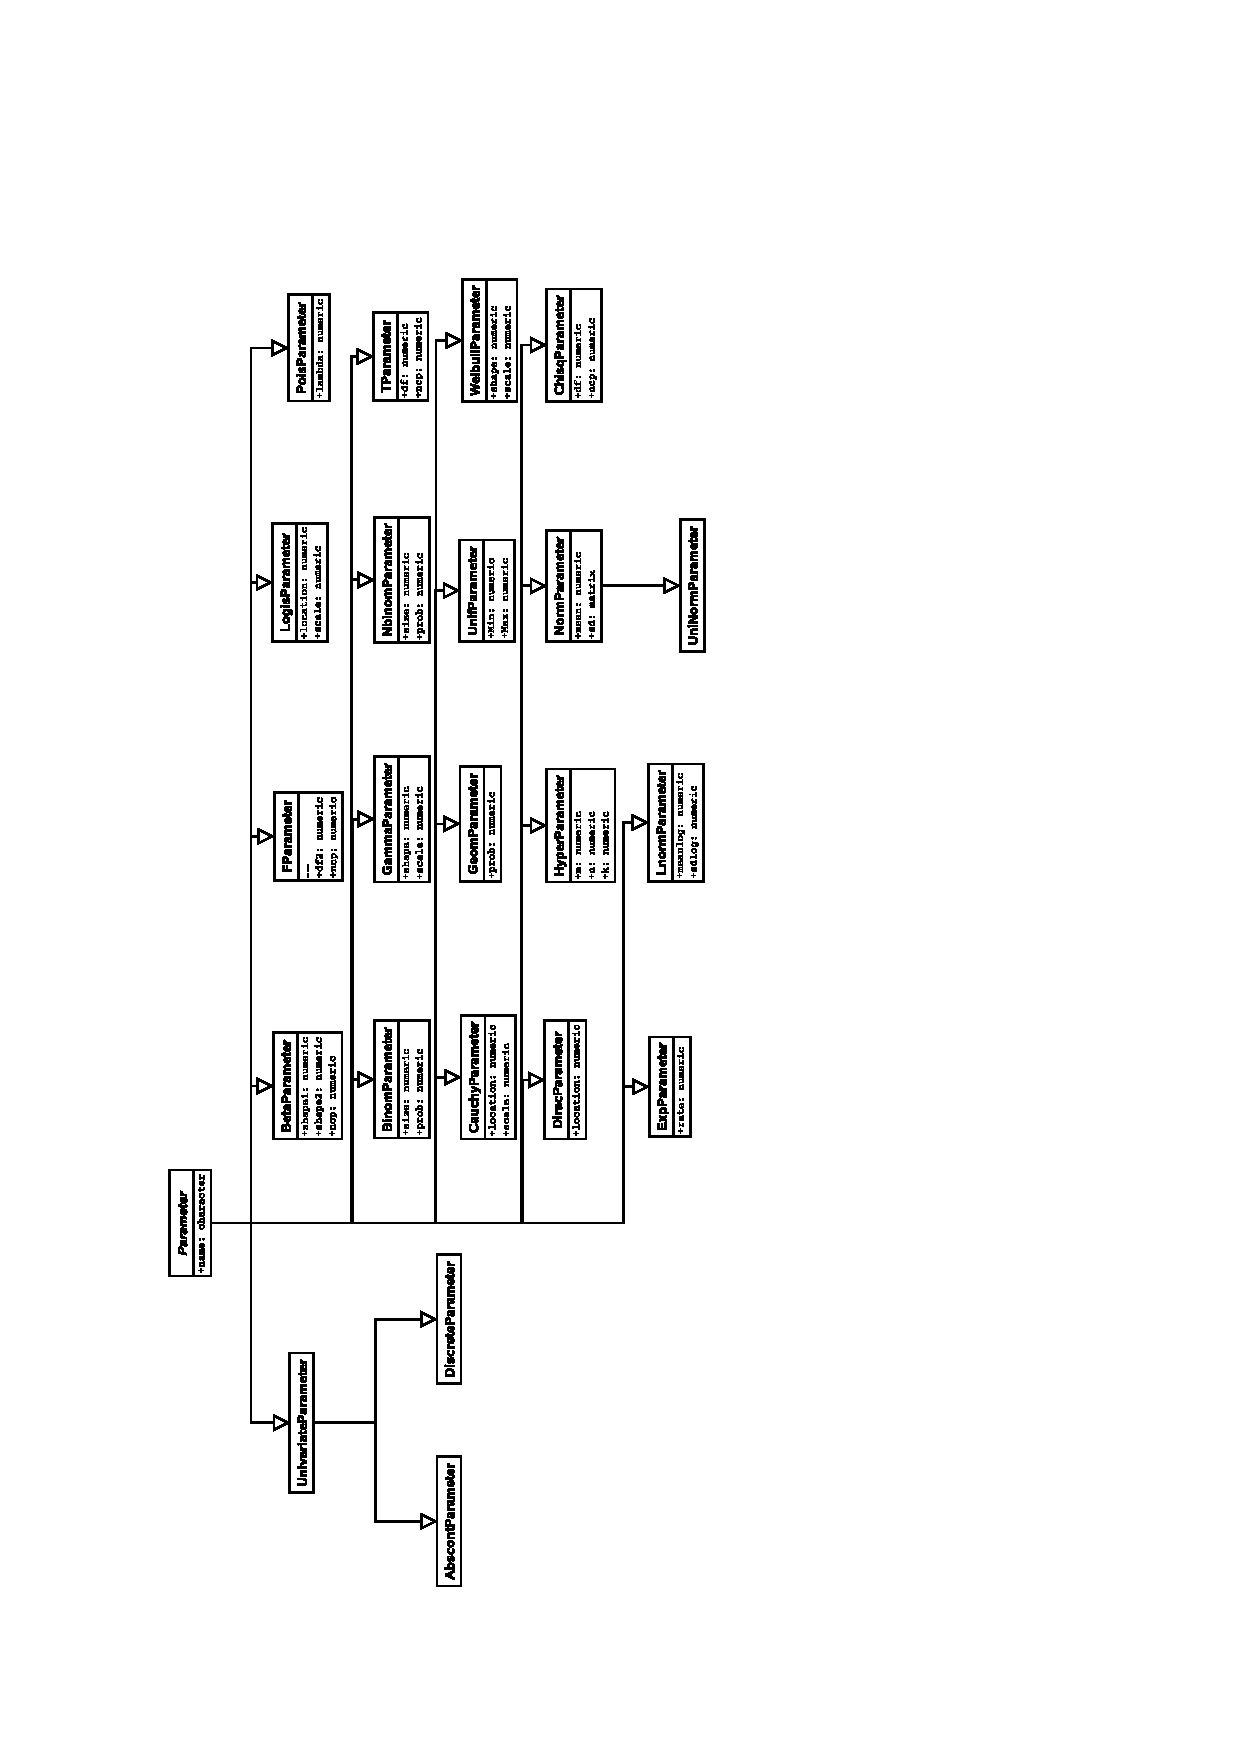
\includegraphics[viewport=30 10 540 390,height=11cm,width=12cm]{parameter.pdf}
% [viewport=30 10 540 390,width=12.cm]
  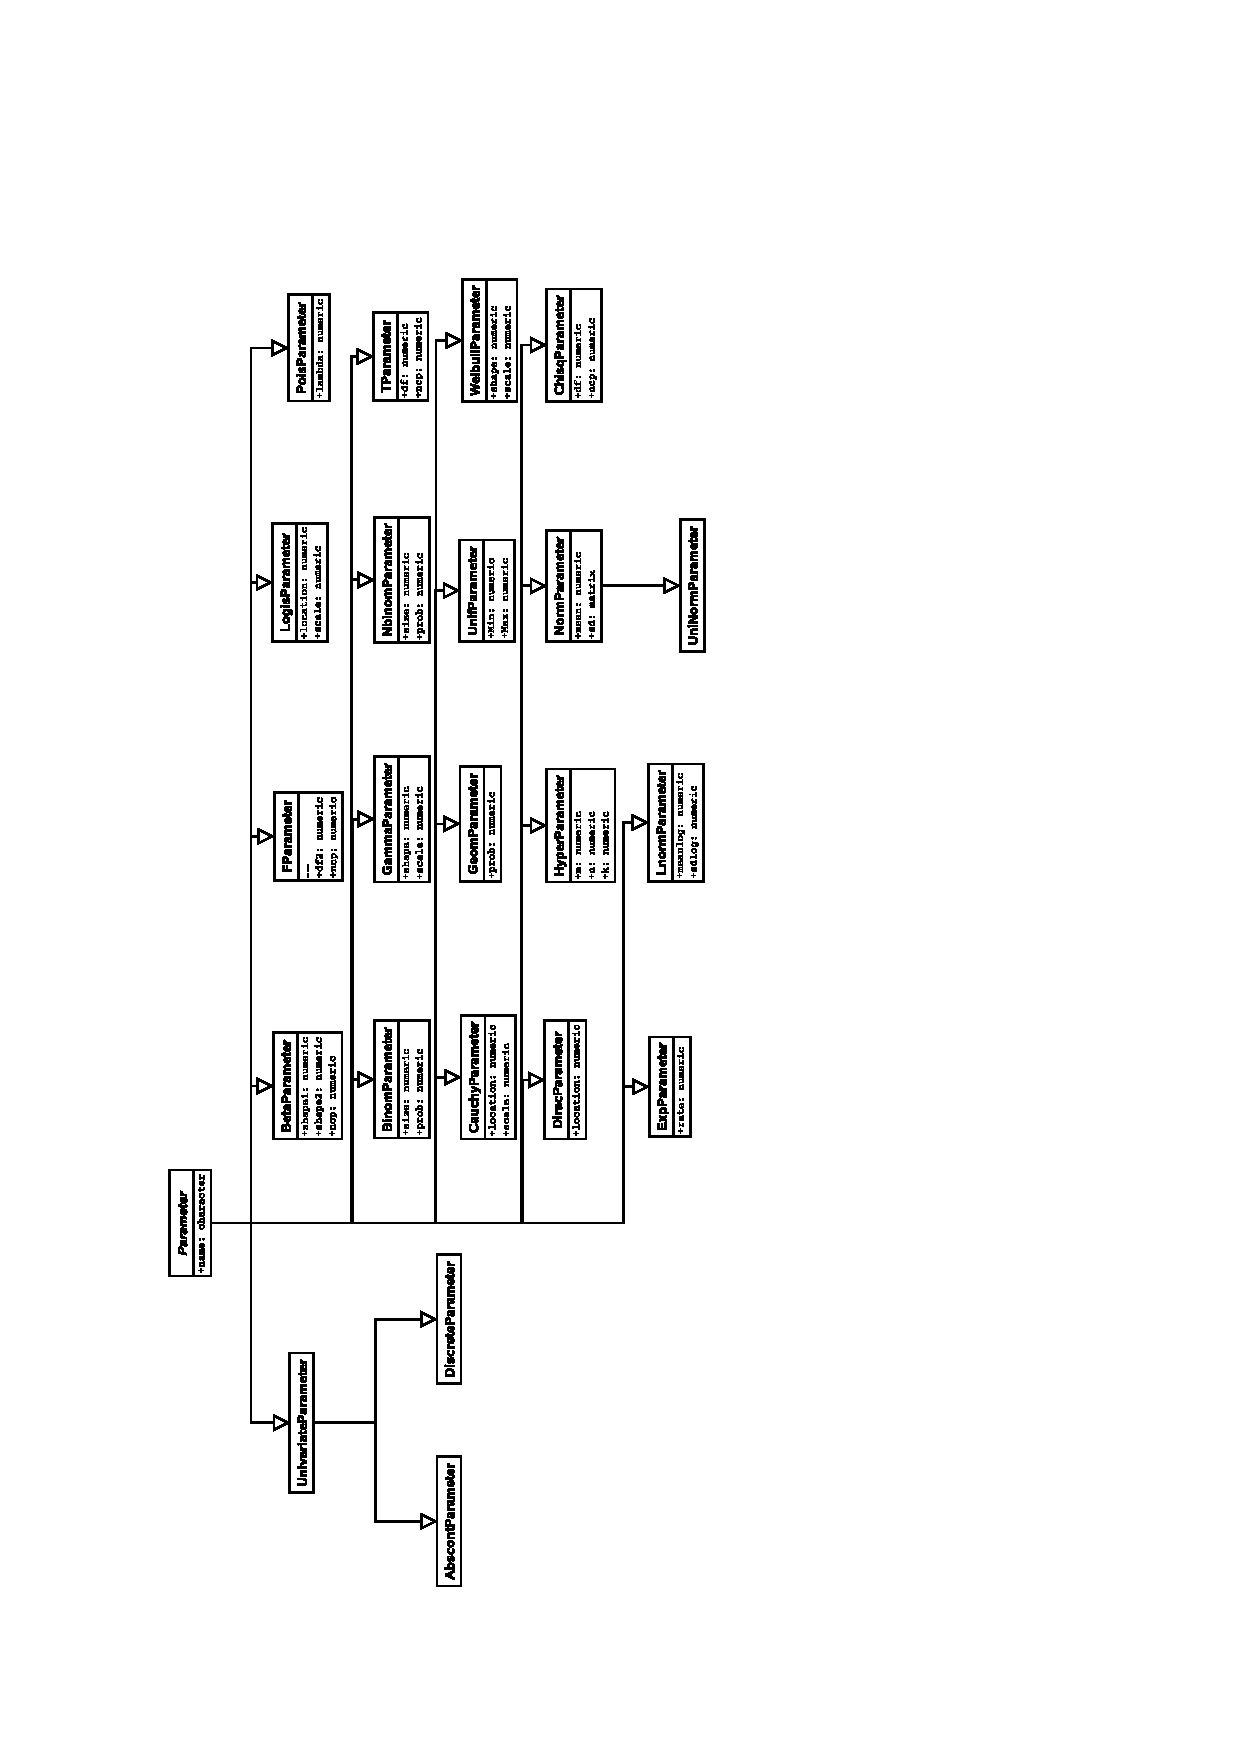
\includegraphics[viewport=30 80 400 690,height=15cm,width=12cm]{parameter.pdf}
    %[viewport=30 10 540 390,width=12.cm]
    \caption{\label{fig4c}{\footnotesize Inheritance relations and slots of the 
     corresponding \mbox{(sub-)}classes for \code{Parameter}
    }}
  \end{center}
\end{figure}
\else
\begin{figure}[htb]\label{fig4}
  \begin{center}
    \includegraphics[viewport=80 120 340 600,height=12.8cm,width=9.0cm, 
                     angle=-90]{parameter.ps}%
    \caption{\label{fig4c}{\footnotesize Inheritance relations and slots of the 
              corresponding \mbox{(sub-)}classes
    for \code{Parameter}
    }}
  \end{center}
\end{figure}
\fi
%
The most important set to be used as parameter domain/sample space
 (\code{rSpace}) will be an Euclidean space. So \code{rSpace} and 
 \code{EuclideanSpace} are also implemented as classes,
 the structure of which may be read off in figure~\ref{fig5c}.
\begin{figure}[htb]\label{fig5}
  \begin{center}
    \ifpdf
    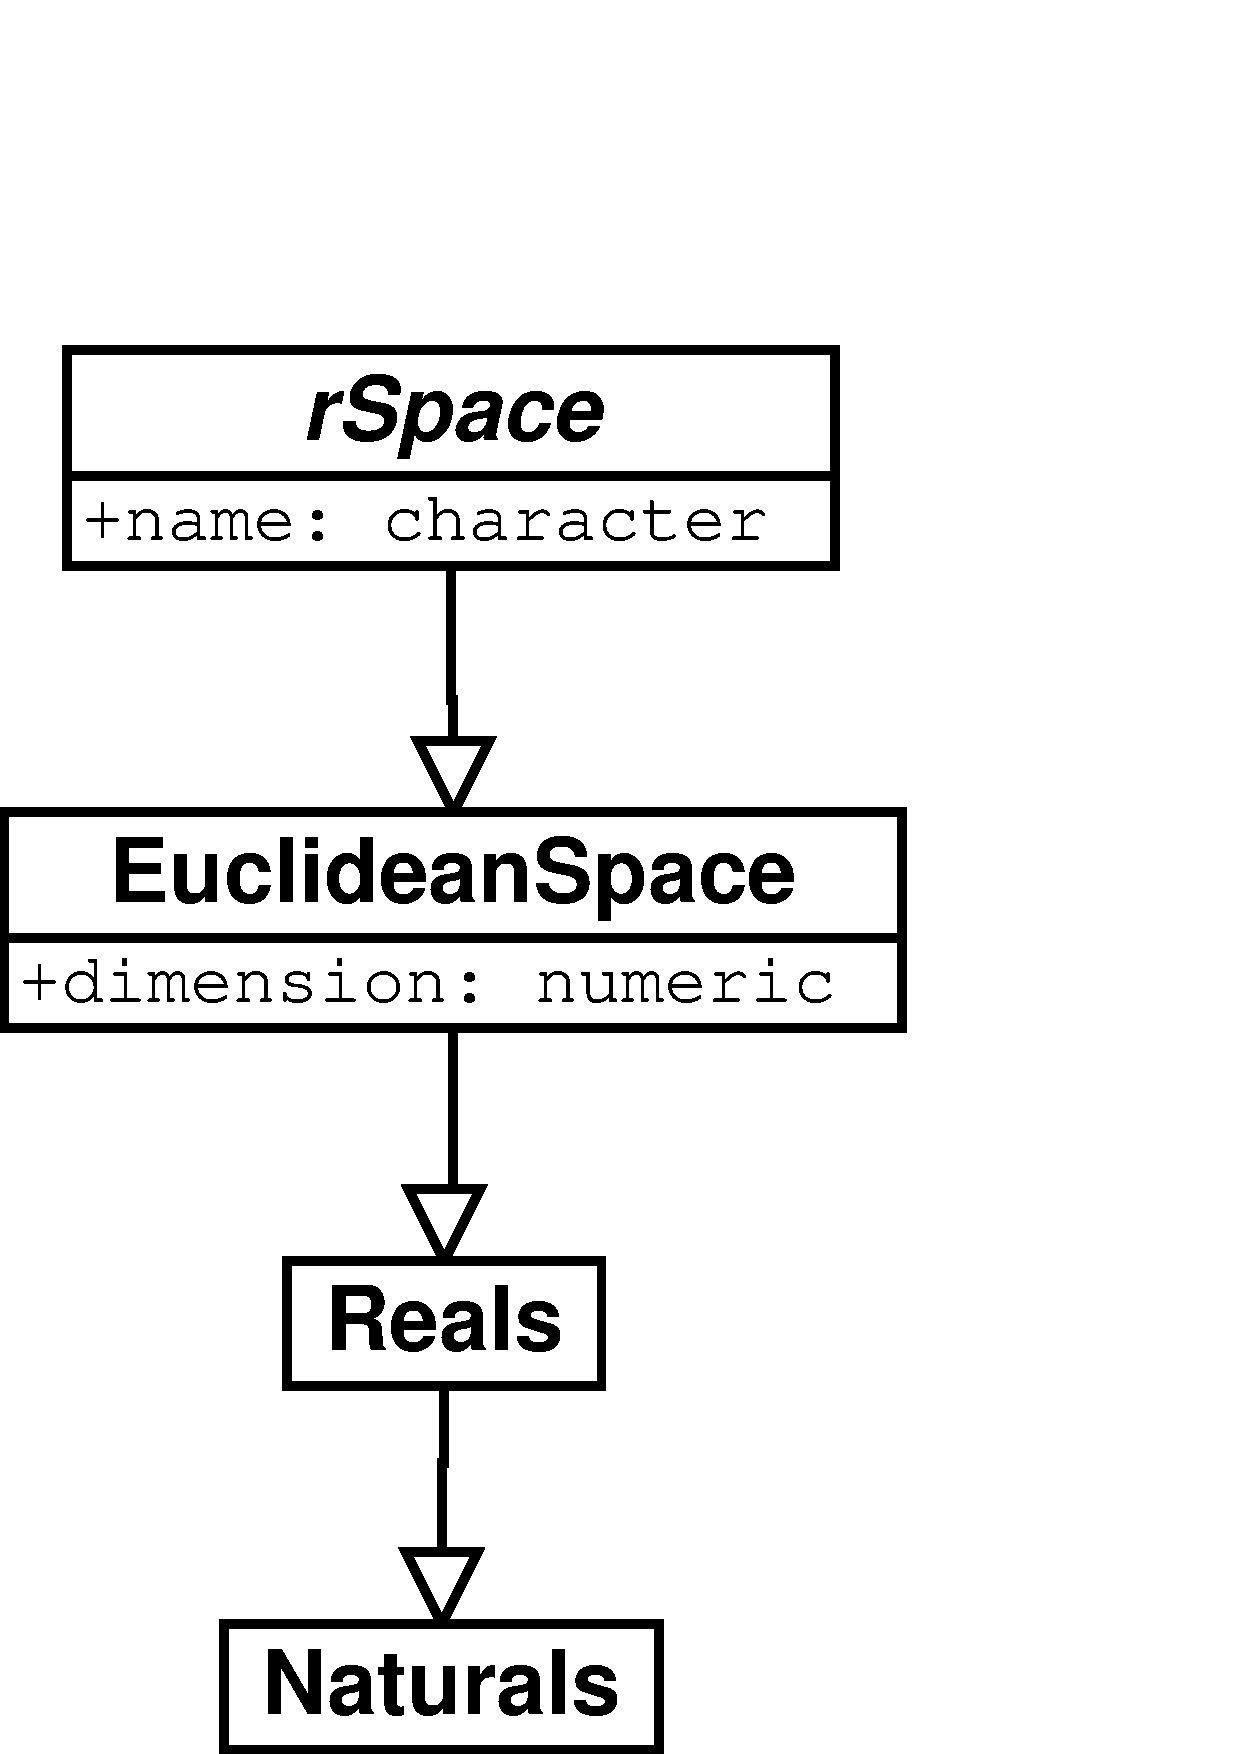
\includegraphics[%viewport=0 30 600 600,
    width=3.9cm]{rspace.pdf}
    \else
    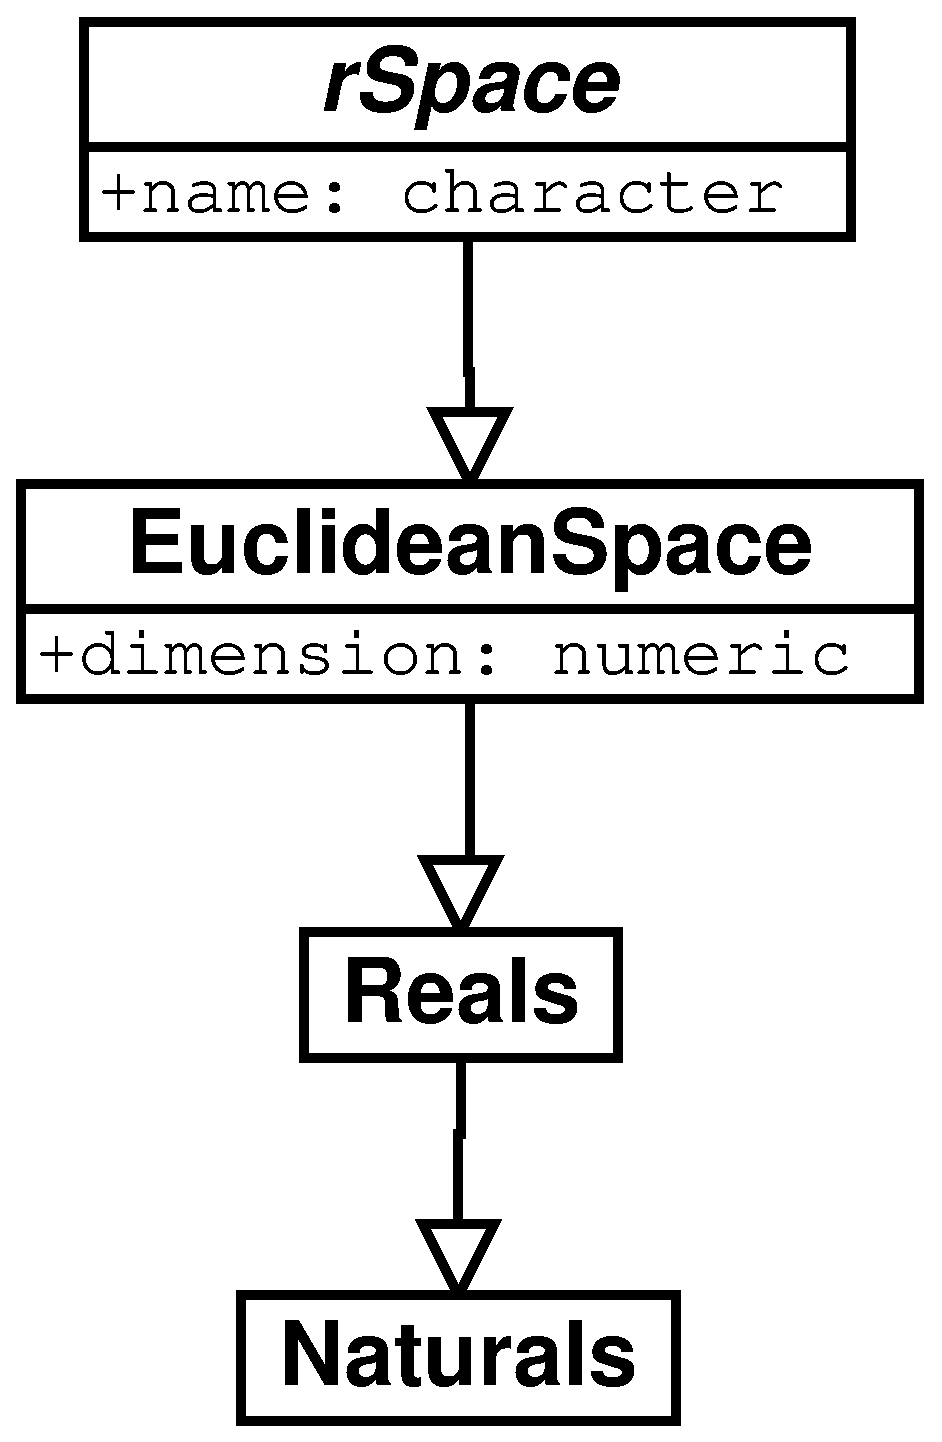
\includegraphics[width=3.7cm]{rspace.ps}%
    \fi
    \caption{\label{fig5c}{\footnotesize Inheritance relations and slots of the 
    corresponding \mbox{(sub-)}classes
    for \code{rSpace}
    }}
  \end{center}
\end{figure}

From version 1.9 on, we also have a subclass \code{Lattice}, which is still 
lacking in the preceding figure. It has slots \code{pivot} (of class 
"numeric"), \code{width} (of class "numeric" but tested against ``{\tt ==0}'')
and  \code{Length} (of class "numeric" but tested to be an integer 
``{\tt >0}'' or {\tt Inf}). 
All slots may be inspected/modified by the usual accessor/replacement functions.

\subsection{Simulation classes}
From version 1.6 on, the classes and methods of this subsection are available in 
package  \pkg{distrSim}.

The aim of simulation classes is to gather all relevant information about a 
simulation in a correspondingly designed class. To this end we introduce the 
class \code{Dataclass} that serves as a common mother class for both "real" and 
simulated data.
%
As derived classes we then have a simulation class where we also gather all 
information needed to reconstruct any particular simulation.\\
%
%\newline0??????\\
From version 1.8 of this package on, we have changed the
format how data / simulations are stored:
In order to be able to cope with multivariate,
regression  and (later) time series distributions,
we have switched to the common array format
%
{\tt samplesize x obsDim x runs} where {\tt obsDim} is the dimension of the 
observations.
%
For saved objects from earlier versions, we provide the functions
\code{isOldVersion} and \code{conv2NewVersion} to check whether the
object was generated by an older version of this package and
to convert such an object to the new format, respectively.
For objects generated from version 1.8 on, you get the package 
version of package~\pkg{distrSim}, under which they have been generated
by a call to \code{getVersion()}. \\
%
%??????1\\
 Finally, coming from robust statistics
we also consider situations where the majority of the data stems from an ideal 
situation/distribution whereas a minority comes from a contaminating source. To 
be able to identify ideal and contaminating observations, we also store this 
information in an indicator variable.\\
%
As the actual values of the simulations only play a secondary role, and as the 
number of simulated variables can become very large, but still easily 
reproducible, it is not worth storing all simulated observations but rather only 
the information needed to reproduce the simulation.
This can be done by \code{savedata}.\\
Schematically, the inheritance relations of class \code{Dataclass} as well as 
the slots of the corresponding \mbox{(sub-)}classes may be read off in 
figure~\ref{fig2c} where we do not  repeat inherited slots.
\begin{figure}[htb]\label{fig2}
  \begin{center}
    \ifpdf
    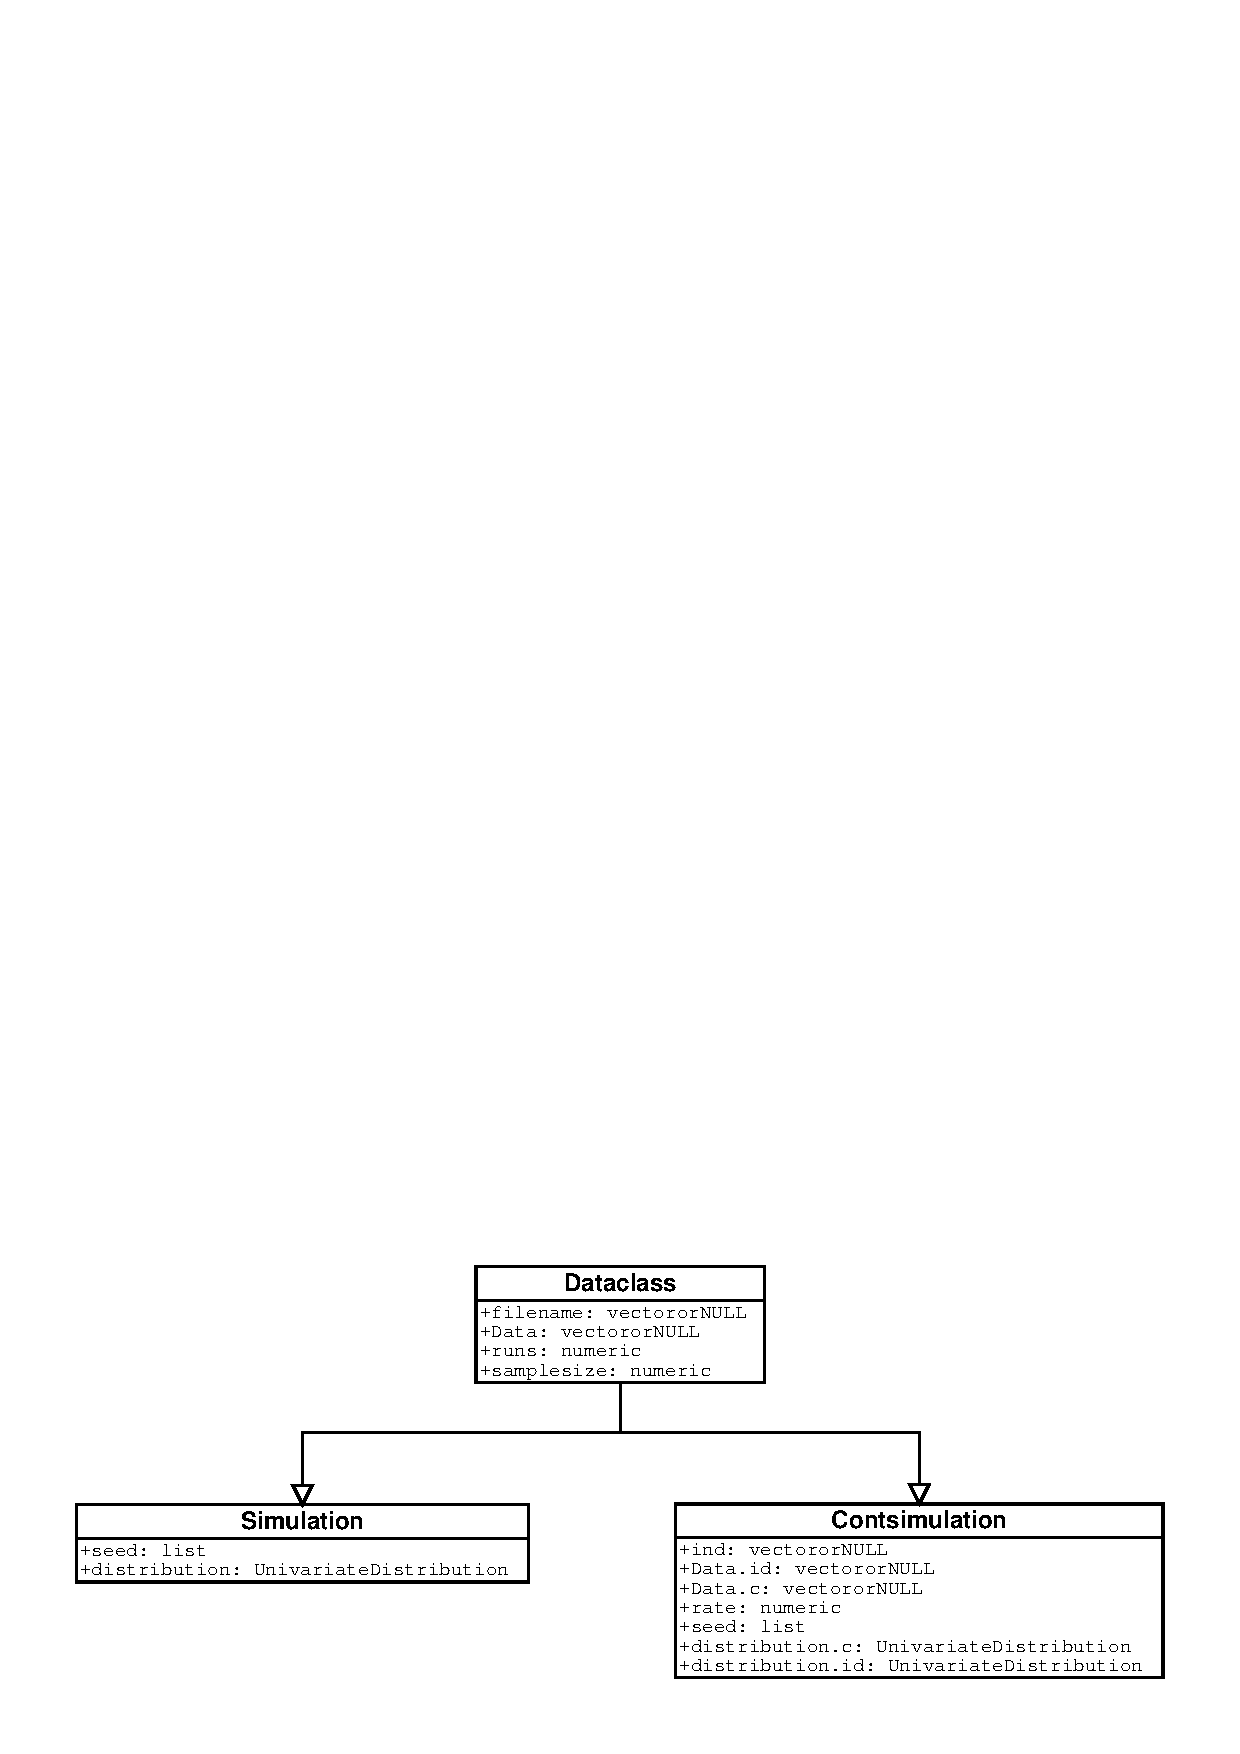
\includegraphics[viewport=120 30 470 250,width=8.5cm]{dataclass.pdf}
    \else
    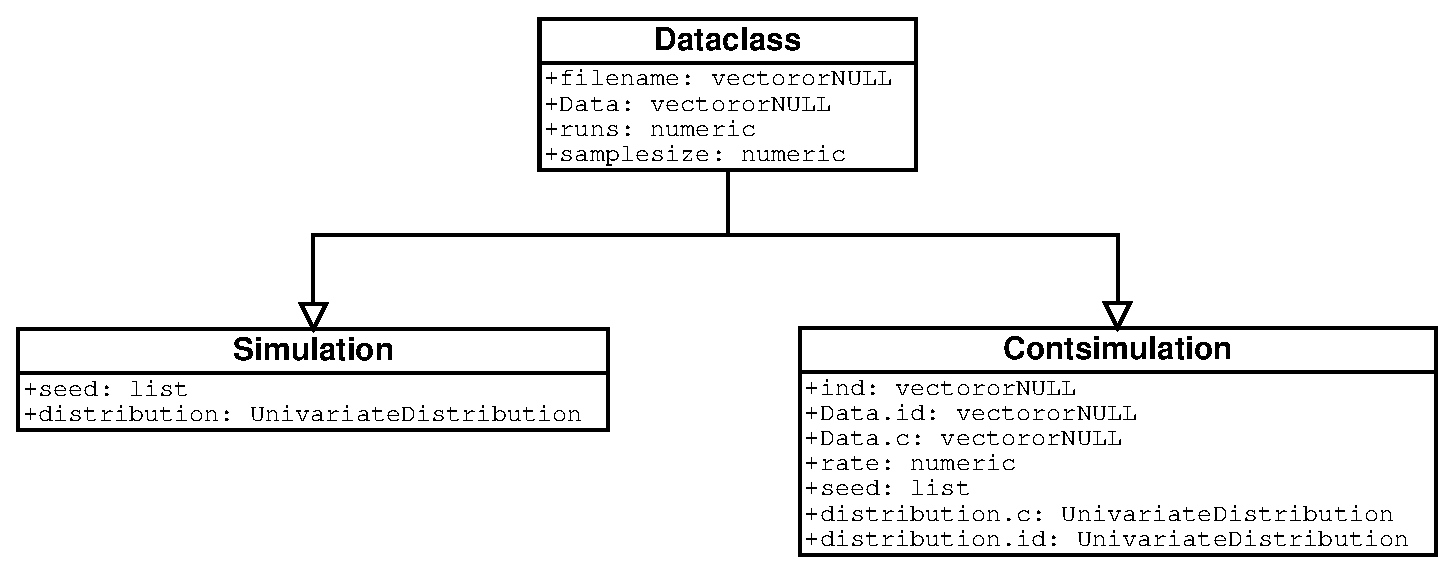
\includegraphics[width=12.5cm]{dataclass.ps}%
    \fi
    \caption{\label{fig2c}{\footnotesize Inheritance relations and slots of the 
    corresponding \mbox{(sub-)}classes
    for \code{Dataclass}
    }}
  \end{center}
\end{figure}
%\newline0??????\\
Also, analogously to  package %s
 \pkg{distr}, %and \pkg{distrEx},
 global options for the output by methods \code{plot} and \code{summary}
are controlled by \code{distrSimoptions()} and \code{getdistrSimoptions()}
\smallskip\\
%??????1\\

\subsection{Evaluation class}
From version 1.6 on, the class and methods of
this subsection are available in package  \pkg{distrTEst}. \\
When investigating properties of a new procedure (e.g. an estimator) by means of 
simulations, one typically evaluates this procedure on a large set of simulation 
runs and gets a result for each run. These results are typically not available 
within seconds, so that it is worth storing them.
To organize all relevant information about these results, we introduce a class 
\code{Evaluation} the slots of which is filled by method \code{evaluate} ---see 
subsection~\ref{evaluate}. Schematically, the slots of this class may be read 
off in figure~\ref{fig3c}.
\begin{figure}[htb]\label{fig3}
  \begin{center}
    \ifpdf
    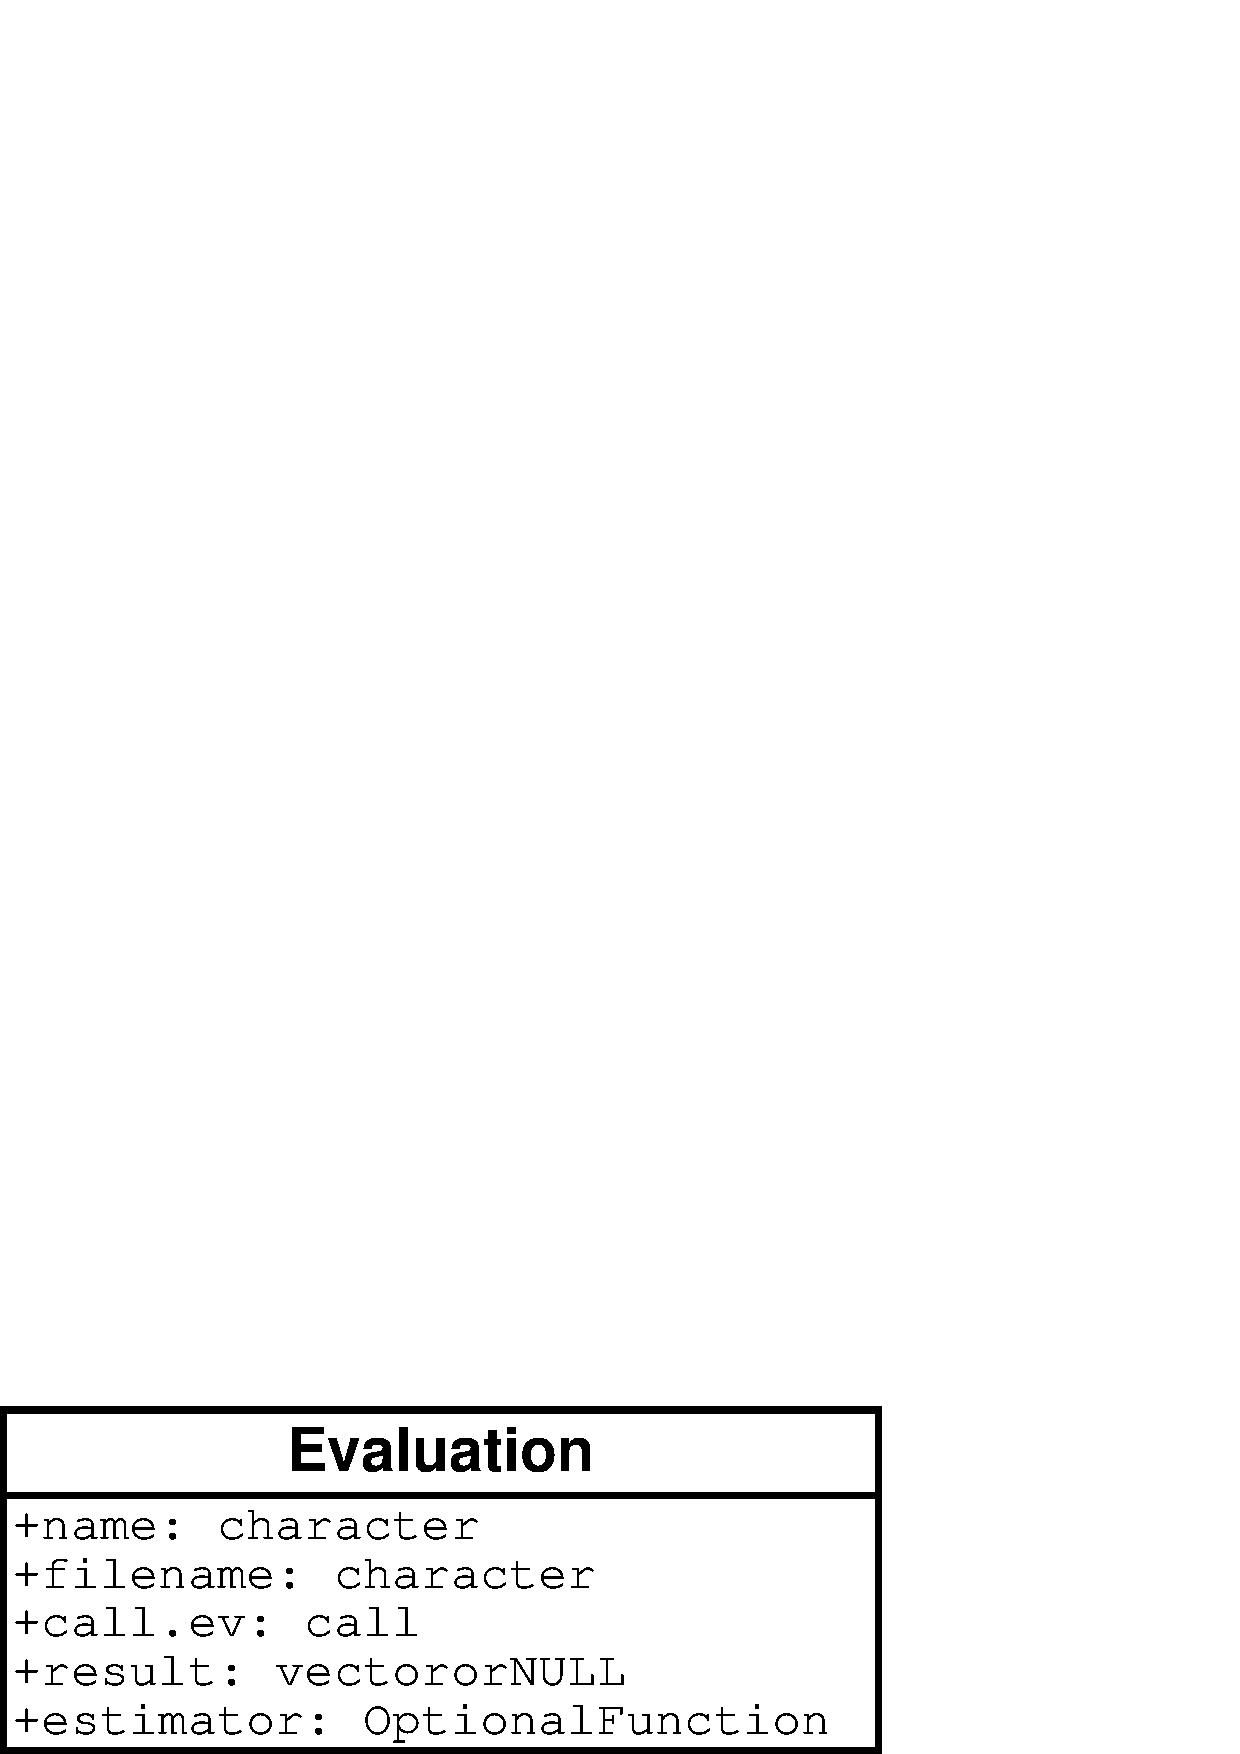
\includegraphics[viewport=60 20 420 200,width=5cm]{evaluation.pdf}
    \else
    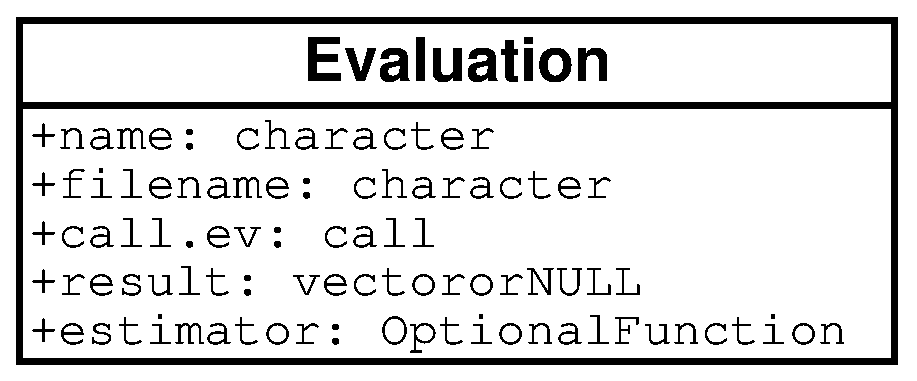
\includegraphics[width=5cm]{evaluation.ps}%
    \fi
    \caption{\label{fig3c}{\footnotesize Slots of class \code{Evaluation}}}
  \end{center}
\end{figure}
%\newline0??????\\
A corresponding \code{savedata} method
saves the object of class \code{Evaluation} in two files in the {\sf R}-working 
directory: one using the filename \code{<filename>} also stores the results; the 
other one, designed to be ``human readable'', comes as a comment file with 
filename \code{<filename>.comment}
only stores the remaining information.
The filename can be specified in the optional argument \code{fileN} to 
\code{savedata}; by default it is concatenated from the \code{filename} slot of 
the \code{Dataclass} object and \code{<estimatorname>}, which you may either
pass as argument \code{estimatorName} or by default is taken as the {\sf R}-name 
of the corresponding {\sf R}-function specified in slot \code{estimator}.

From version 1.8 on, slot \code{result} in class \code{Evaluation} is of class 
\code{DataframeorNULL}, i.e.; may be either a data frame or {\tt NULL}, and slot 
\code{call.ev} in class \code{Evaluation} is of class "CallorNULL", i.e.; may be 
either a call or {\tt NULL}. Also, we want to gather \code{Evaluation} objects 
in a particular data structure \code{EvaluationList}
(see below), so we have to be able to check whether all data sets in the 
gathered objects coincide.
For this purpose, from this version on, class \code{Evaluation} has an 
additional slot \code{Data} of class \code{Dataclass}. In order not to burden 
the objects of this class too heavily with uninformative
simulated data, in case of a slot \code{Data} of one of the simulation-type 
subclasses of \code{Dataclass},
this \code{Data}  itself has an empty \code{Data}-slot.\\

\subsection{EvaluationList class}
The class and methods of this subsection are available in package 
 \pkg{distrTEst}. \\
In order to compare different procedures / estimators for the
same problem, it is natural to gather several \code{Evaluation} objects
with results of the same range (e.g.\ a parameter space) generated on the
same data, i.e.; on the same \code{Dataclass} object. To this end, from
version 1.8 on, we have introduced class \code{EvaluationList}.
Schematically, the slots of this class may be read off in figure~\ref{fig3c1}.
\begin{figure}[htb]\label{fig3-1}
  \begin{center}
    \ifpdf
    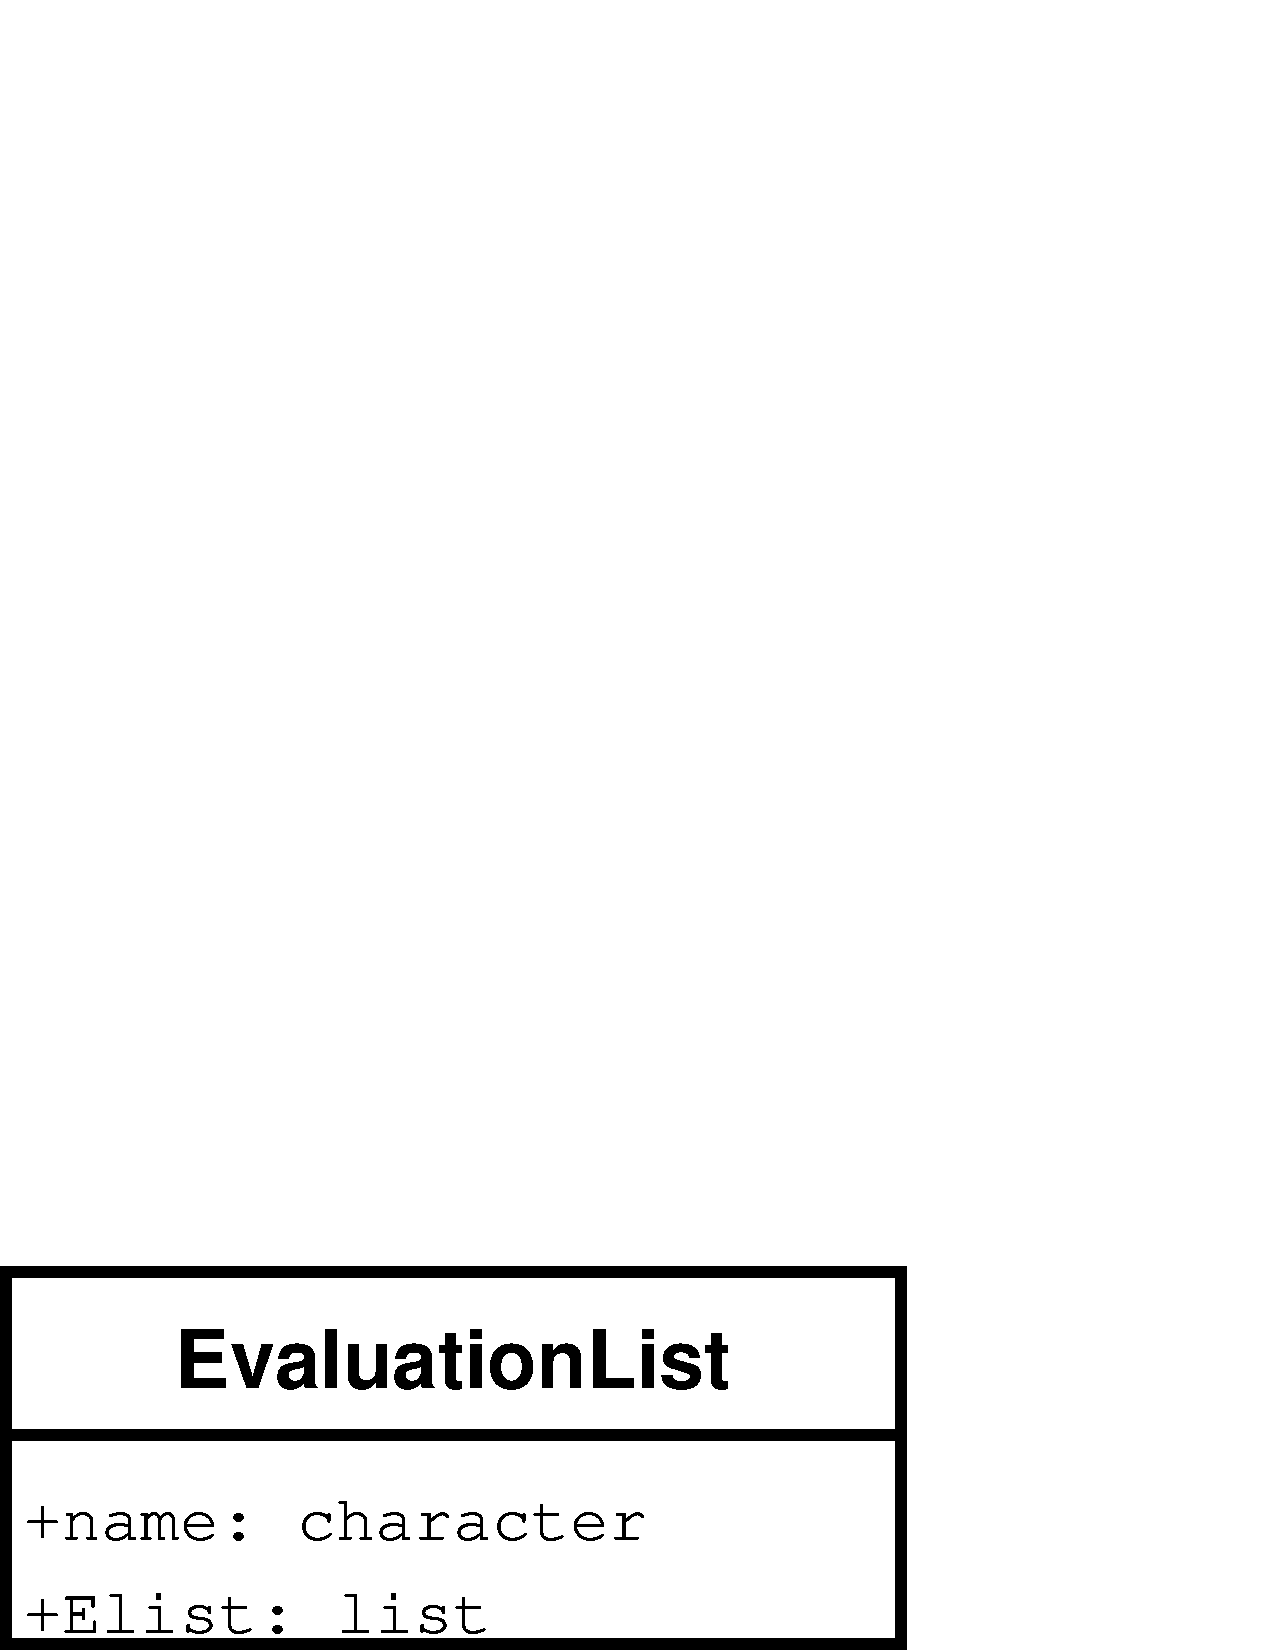
\includegraphics[viewport=0 0 436 185,width=5.5cm]{EvaluationList.pdf}%
    \else
    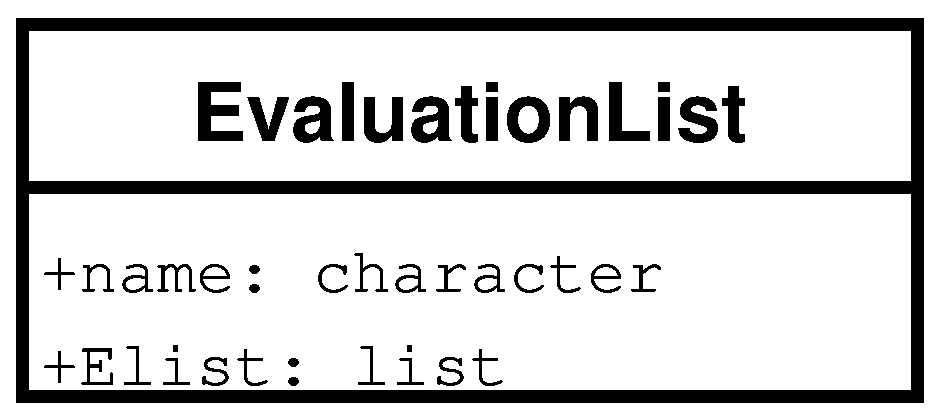
\includegraphics[viewport=0 0 436 185,width=5.5cm]{EvaluationList.ps}%
    \fi
%\parbox{10cm}{TO BE DONE}
    \caption{\label{fig3c1}{\footnotesize Slots of class \code{EvaluationList}}}
  \end{center}
\end{figure}
The common \code{Data} slot of the \code{Evaluation} objects in an 
\code{EvaluationList} object may be accessed by the accessor method \code{Data}.
%??????1\\
%
%
\section{Methods}\label{methods}
%
We have made available quite general arithmetical operations to our distribution 
objects, generating new image distributions automatically.

\begin{description}
  \item[{\Large \sc Caveat:\/}] {\bf These arithmetics
operate on the corresponding r.v.'s and {\bf not} on the distributions.}
\end{description}
(For the latter, they only would make sense in restricted cases like convex 
 combinations).\\

Martin M\"achler pointed out that this might be confusing. So, this warning is 
also issued on attaching package \pkg{distr}, and,  by default, again whenever a 
\code{Distribution} object, produced by such arithmetics is shown or printed; 
this also applies to the last line in
\begin{Schunk}
\begin{Sinput}
>   A1 <- Norm(); A2 <- Unif()
>   A1 + A2
\end{Sinput}
\begin{Soutput}
Distribution Object of Class: AbscontDistribution
\end{Soutput}
\end{Schunk}
\begin{verbatim}
Warning message:
arithmetics on distributions are understood as operations on r.v.'s
see 'distrARITH()'; for switching off this warning see '?distroptions' in: 
print(object)
\end{verbatim}
This behaviour will soon be annoying so you may switch it off setting the global 
option
\code{WarningArith} to \code{FALSE} (see section~\ref{options}).
%
\subsection{Affine linear transformations}\label{afflin}
%
We have overloaded the operators \code{"+"}, \code{"-"}, \code{"*"}, \code{"/"} 
such that affine linear transformations which involve only single univariate 
r.v.'s are available;
i.e.\ is expressions like \code{Y=(3*X+5)/4} are permitted for an object 
\code{X} of class \code{AbscontDistribution}
or \code{DiscreteDistribution}
(or some subclass), giving again an object \code{Y} of
class \code{AbscontDistribution} or \linebreak[4]\code{DiscreteDistribution} 
(in general). 
Here the corresponding transformations of the \code{d}, \code{p}, and 
\code{q}-functions are done analytically.\\
%
From version 1.9 on, we use subclasses 
\code{AffLinAbscontDistribution}, \code{AffLinDiscrete\-Distribution},
\code{AffLinLatticeDistribution} as classes of the return values to enhance
accuracy of functinals like \code{E}, \code{var}, etc.\ 
in package \pkg{distrEx}. These classes in addition
to their counterparts without prefix ``\code{AffLin}'' have slots \code{a}, \code{b},
and \code{X0}, to capture the fact that an object of this class is distributed
as \code{a * X0 + b}. Also, we introduce a class union \code{AffLinDistribution}
of classes \code{AffLinAbscontDistribution} and
\linebreak[4]\code{AffLinDiscrete\-Distribution}.
Consequently, the result \code{Y} of \code{Y <- a1 * X + b1} for an 
object \code{X} of (a subclass of) class \code{AffLinDiscrete\-Distribution}
(if \code{ a != 0}) is of the same class as \code{X} but with slots
\code{Y@a = a1 * X@a}, \code{Y@b = b1 + X@b}, \code{Y@X0 = X@X0}.
%
\subsection[The group math of unary mathematical operations]{The group 
\code{math} of unary mathematical operations}
%
Also the group \code{math} of unary mathematical operations is available for
distribution classes; so
expressions like \code{exp(sin(3*X+5)/4)} are permitted.
%
 The corresponding \code{r} method consists in simply
performing the transformation to the simulated values of \code{X}.
The corresponding (default-) \code{d}, \code{p} and \code{q}-functions are 
obtained by simulation, using the technique described in the following 
subsection.\\
By means of \code{substitute}, the bodies of the \code{r}, \code{d}, 
\code{p}, \code{q}-slots of distributions show the parameter values with 
which they were generated; in particular,
convolutions and applications of the group \code{math} may be traced in
the \code{r}-slot of a distribution object, compare\newline
\code{r(sin(Norm()) + cos(Unif() * 3 + 2))}.

Initially, it might be irritating that the same ``arithmetic'' expression
evaluated twice in a row gives two different results, compare
\begin{Schunk}
\begin{Sinput}
>   A1 <- Norm(); A2 <- Unif()
>   d(sin(A1 + A2))(0.1)
\end{Sinput}
\begin{Soutput}
[1] 0.3761359
\end{Soutput}
\begin{Sinput}
>   d(sin(A1 + A2))(0.1)
\end{Sinput}
\begin{Soutput}
[1] 0.3795761
\end{Soutput}
\begin{Sinput}
>   sin(A1 + A2)
\end{Sinput}
\begin{Soutput}
Distribution Object of Class: AbscontDistribution
\end{Soutput}
\end{Schunk}
This is due to the fact, that all slots are filled starting from simulations.
To explain this, a warning is issued  by default, whenever a \code{Distribution}
object, filled by such simulations is shown or printed; this also applies to the 
last line in the preceding code sniplet. This behaviour may again be switched 
off by setting the global option
\code{WarningSim} to \code{FALSE} (see section~\ref{options}).\\

As they are frequently needed, from version 1.9 on, math operations 
\code{abs()}, \code{exp()}, and ---if an {\sf R}-version $\ge$ {\tt 2.6.0} is 
used--- also \code{log()} are implemented in an analytically exact form, 
i.e.; with exact expressions for slots \code{d}, \code{p}, and \code{q}.

%
\subsection{Construction of \code{d}, \code{p}, and \code{q} from \code{r}}
%
In order to facilitate automatic generation of new distributions, in particular 
those arising as image distributions under transformations of correspondingly 
distributed random variables, we provide ad hoc methods that should be 
overloaded by more exact ones wherever possible: By means of the function 
\code{RtoDPQ} we first generate $10^{\footnotesize\tt RtoDPQ.e}$
random numbers where \code{RtoDPQ.e} is a global option of this package and is 
discussed in section~{\ref{options}}. %
A density estimator is evaluated along this sample, the distribution function is 
estimated by the empirical c.d.f. and, finally, the quantile function is 
produced by numerical inversion.
Of course the result is rather crude as it relies on the law of large numbers 
only, but this way all transformations within the group \code{math} become 
available.
Where laws under transformations can easily be computed exactly ---as for affine
linear transformations--- we replace this procedure by the exactly transformed
\code{d}, \code{p}, \code{q}-methods.
%
\subsection{Convolution}
%
A convolution method for two independent r.v.'s is implemented by means 
of explicit calculations for discrete summands, and by means of 
DFT/FFT\footnote{Details to be found in \cite{K:R:S:04}} if one of the summands is 
absolutely continuous or (from version 1.9 on:) both are lattice distributed 
with a common lattice as support.
This method automatically generates the law of the sum of two independent 
variables/distributions $X$ and $Y$ of any univariate distributions ---or 
in {\tt S4}-jargon: the addition operator \code{"+"} is overloaded for two 
objects of class \code{UnivariateDistribution} and corresponding subclasses.
%
\subsection{Overloaded generic functions}
Methods \code{print}, \code{plot}, \code{show} and \code{summary} have been 
overloaded for classes \code{Distribution}, \code{Dataclass}, \code{Simulation}, 
\code{ContSimulation}, as well as \code{Evaluation} and \code{EvaluationList} to 
produce ``pretty''  output. %\newline 0??????\\
\code{print}, \code{plot}, \code{show} and \code{summary} have additional, 
optional arguments for plotting subsets of the simulations / results:
index vectors for the dimensions, the runs, the observations, and the 
evaluations may be passed using arguments \code{obs0},  \code{runs0}, 
\code{dims0}, \code{eval0}, confer
\code{help("<mthd>-methods",package=<pkg>)} where \code{<mthd>} stands for 
\code{plot}, \code{show}, \code{print}, or \code{plot}, and \code{<pkg>} stands 
for either \pkg{distrSim} or \pkg{distrTEst}.

For an object of class \code{Distribution},
\code{plot} displays the density/probability function, the c.d.f.\ and the 
quantile function of a distribution. Note that all usual parameters of 
\code{plot} remain valid. For instance, you may increase the axis annotations 
and so on. More important, you may also 
override the automatically chosen $x$-region by passing an \code{xlim} argument:
\begin{Schunk}
\begin{Sinput}
>   plot(Cauchy(),withSweave = TRUE)
\end{Sinput}
\end{Schunk}
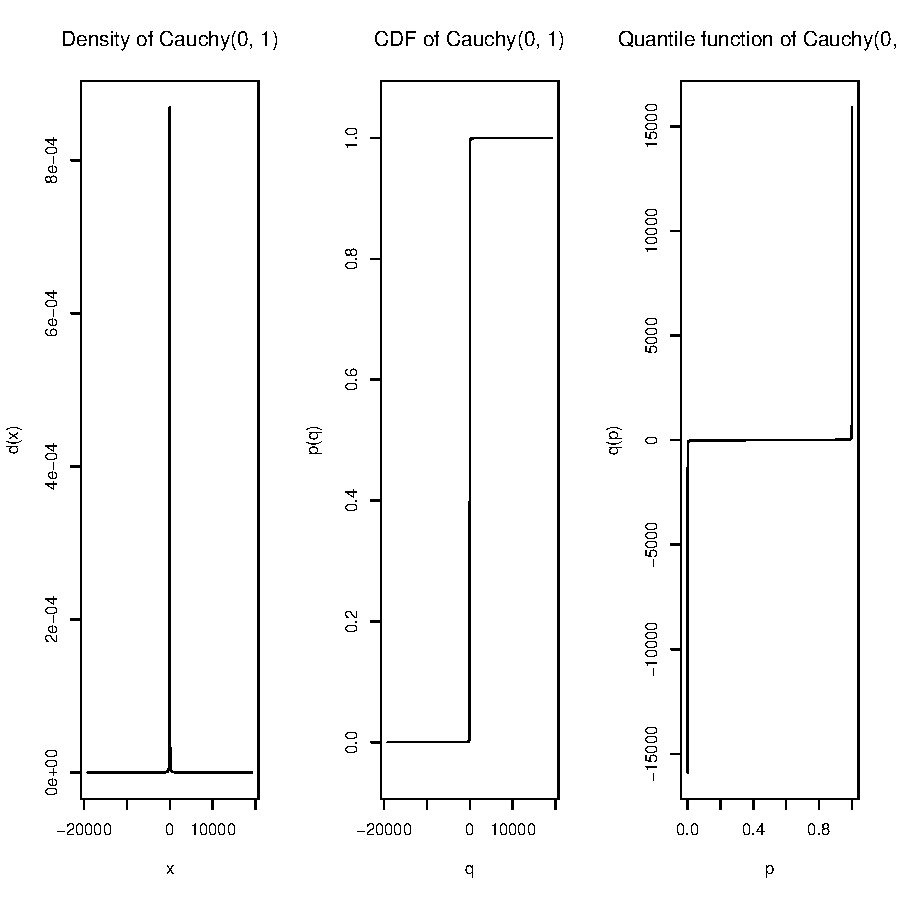
\includegraphics{distr-cauchy1}
\begin{Schunk}
\begin{Sinput}
>   plot(Cauchy(),xlim=c(-4,4),withSweave = TRUE)
\end{Sinput}
\end{Schunk}
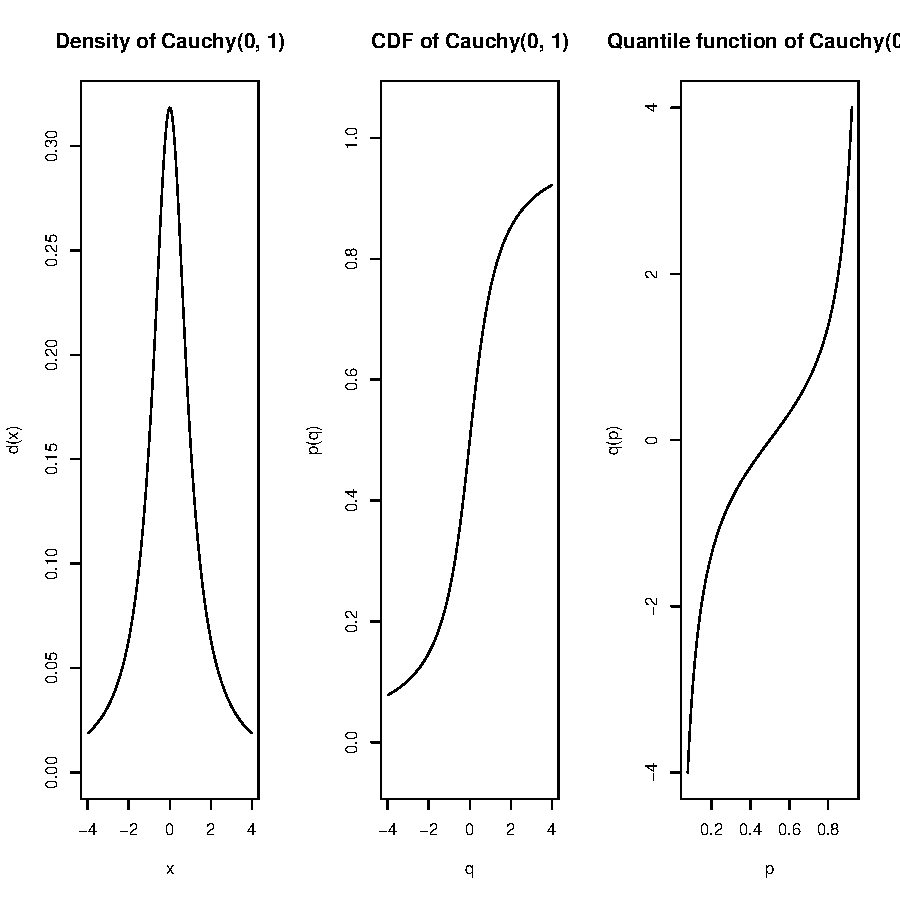
\includegraphics{distr-cauchy2}

Moreover you may control optional main, inner titles and subtitles with 
arguments \code{main} / \code{sub} / \code{inner}. To this end there are 
preset strings substituted in both expression and character vectors 
(where in the following \code{x} denotes the argument 
with which \code{plot()} was called)
\begin{itemize}
 \item[\%A] deparsed argument \code{x}
 \item[\%C] class of argument \code{x}
 \item[\%P] comma-separated list of parameter values of slot \code{param} of 
            argument \code{x}
 \item[\%Q] comma-separated list of parameter values of slot \code{param} of 
            argument \code{x} in parenthesis unless this list is empty; then 
            \code{""}
 \item[\%N] comma-separated {\tt <name> = <value>} - list of parameter values of 
            slot \code{param} of argument \code{x}
 \item[\%D] time/date at which plot is/was generated
\end{itemize}
As usual you may control title sizes and colors with 
\code{cex.main} / \code{cex.inner} / \code{cex.sub} respectively with
\code{col} / \code{col.main} / \code{col.inner} / \code{col.sub}. Additionally
it may be helpful to control top and bottom margins with arguments
\code{bmar}, \code{tmar}. \code{plot()} can also cope with \code{log}-arguments.
We provide different default symbols for unattained [\code{pch.u}] / attained 
[\code{pch.a}] one-sided limits, which may be overridden by corresponding
arguments  \code{pch} / \code{pch.a} / \code{pch.u}.

For objects of class \code{AbscontDistribution}, you may set the number of grid 
points used by an \code{ngrid} argument; also the ``quantile''-panel
takes care of finite left/right endpoints of support and optionally tries
to identify constancy region of the \code{p}-slot. 

For objects of class \code{DiscreteDistributions}, we use \code{stepfun()} from
package \pkg{base} as far as possible and (also for panel ``q'' for
\code{AbscontDistributions}) consequently take over its arguments 
\code{do.points}, \code{verticals}, \code{col.points} / \code{col.vert} / 
\code{col.hor} and \code{cex.points}.

As examples consider the following 10 plots:


\begin{figure}[p]
\begin{Schunk}
\begin{Sinput}
> plot(Binom(size = 4, prob = 0.3), withSweave = TRUE)
\end{Sinput}
\end{Schunk}

\includegraphics{distr-plotex1}
\end{figure}
\begin{figure}[p]
\begin{Schunk}
\begin{Sinput}
> plot(Binom(size = 4, prob = 0.3), do.points = FALSE, verticals = FALSE,
+      withSweave = TRUE)
\end{Sinput}
\end{Schunk}
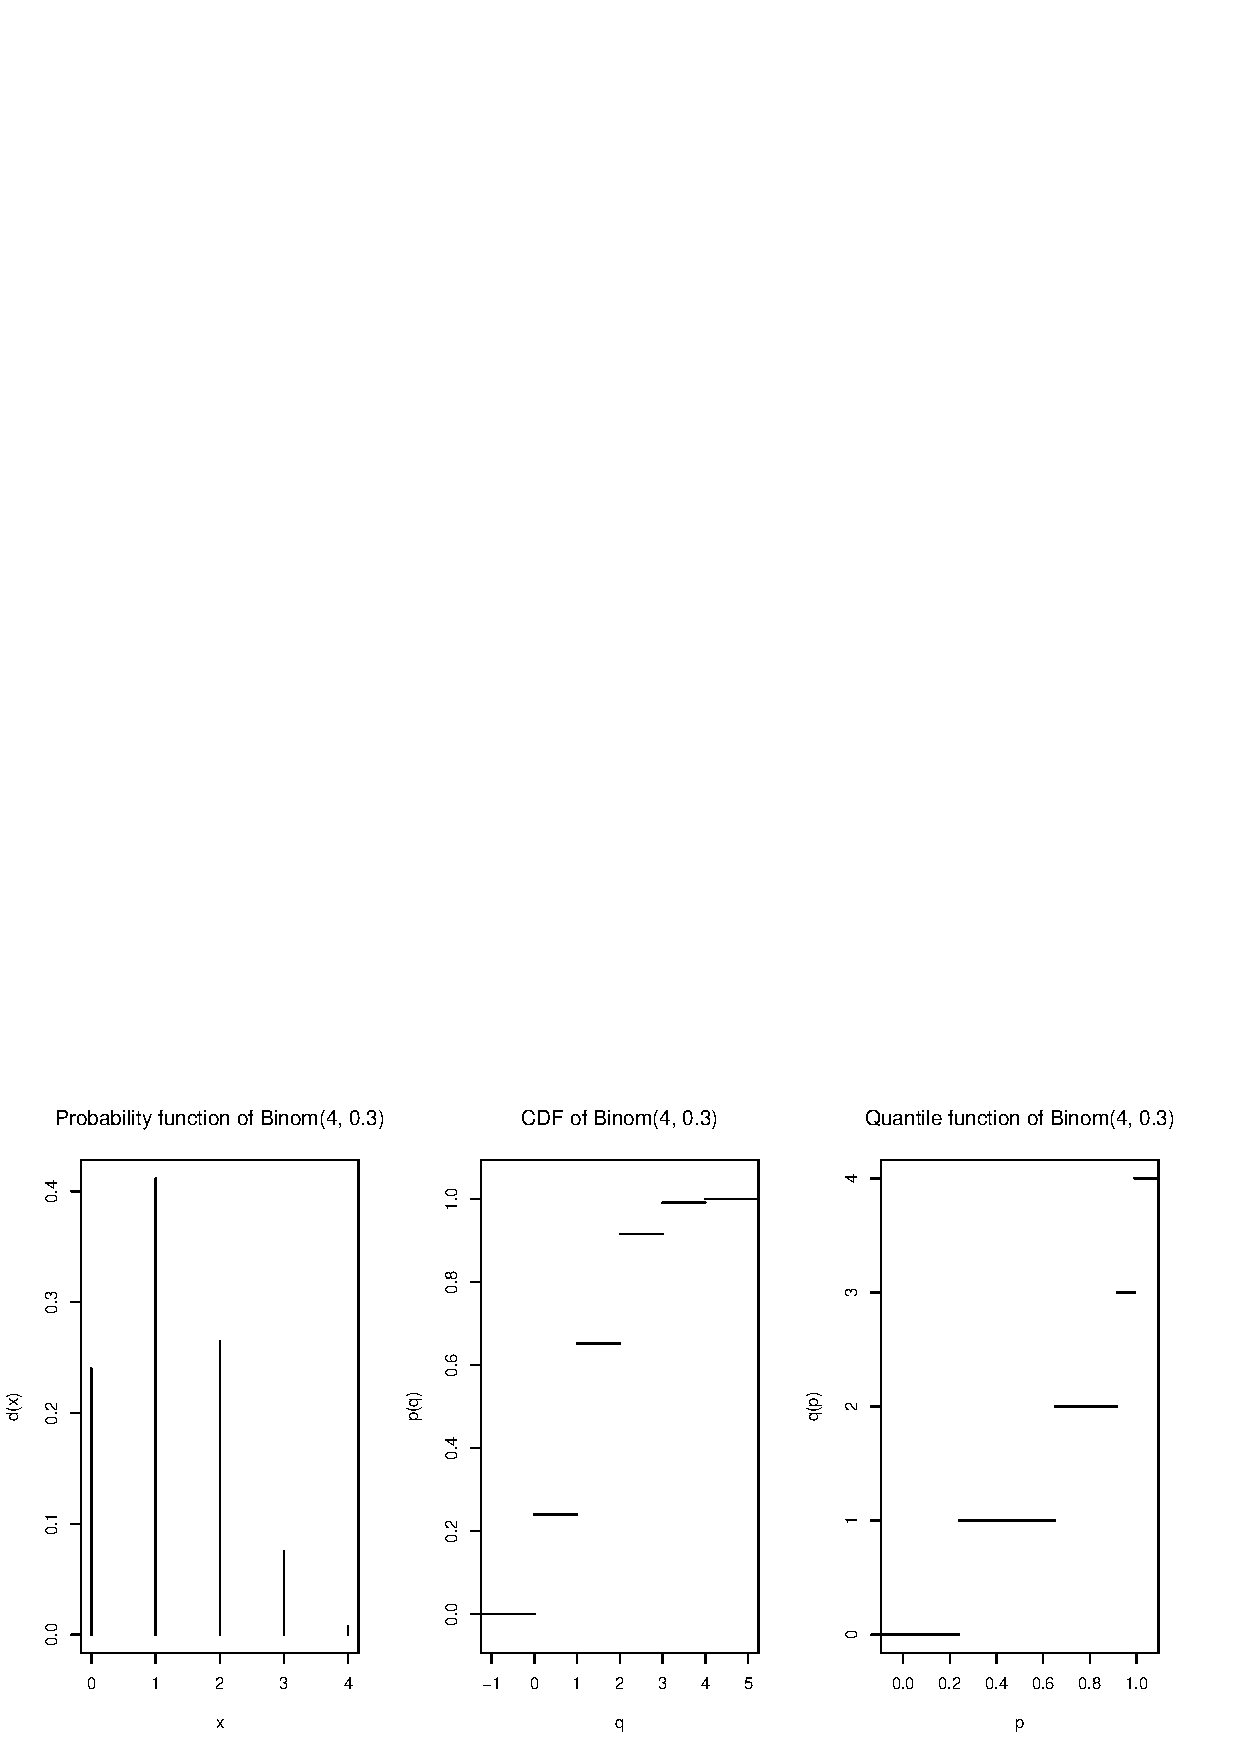
\includegraphics{distr-plotex2}
\end{figure}

\begin{figure}[p]
\begin{Schunk}
\begin{Sinput}
> plot(Binom(size = 4, prob = 0.3), main = TRUE, inner = FALSE, cex.main = 1.6,
+      tmar = 6, withSweave = TRUE)
\end{Sinput}
\end{Schunk}
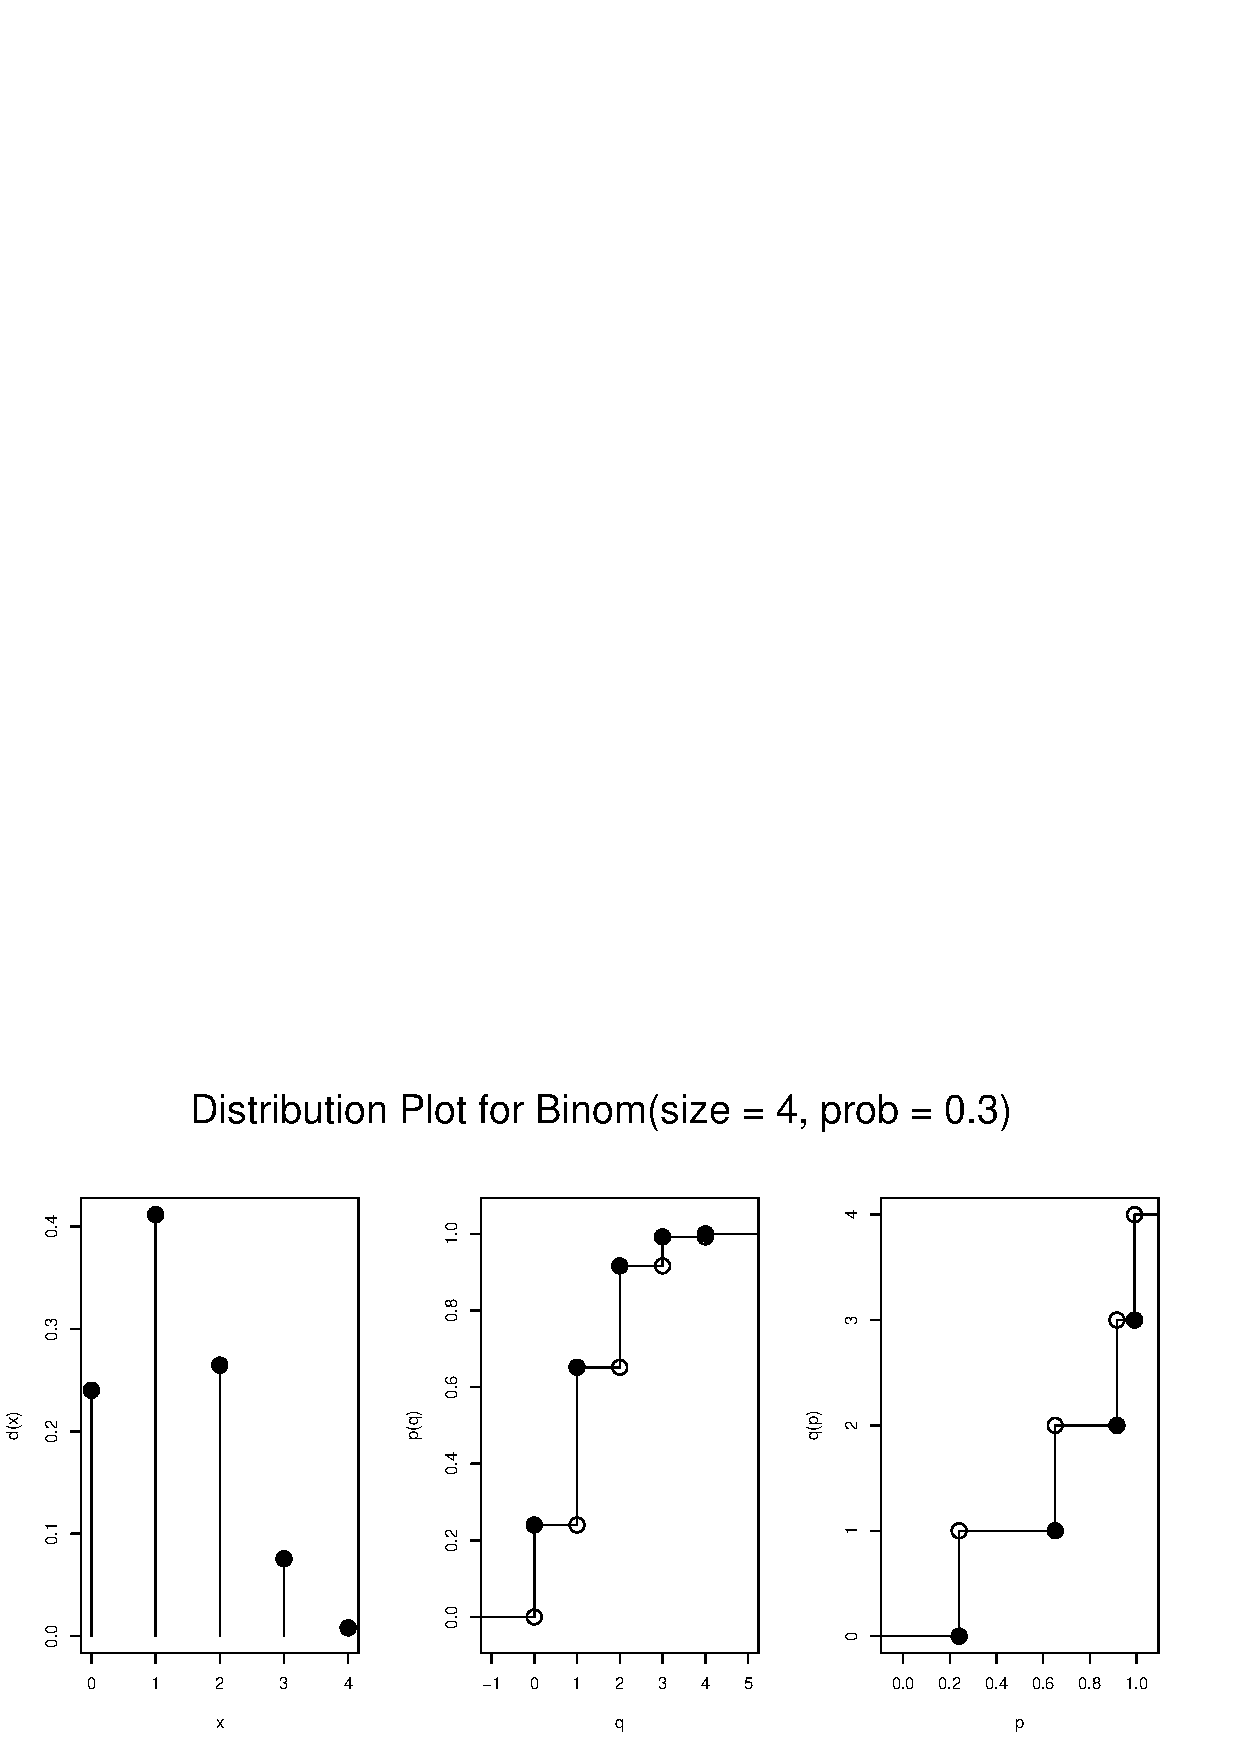
\includegraphics{distr-plotex3}
\end{figure}

\begin{figure}[p]
\begin{Schunk}
\begin{Sinput}
> plot(Binom(size = 4, prob = 0.3), cex.points = 1.2, pch = 20, lwd = 2,
+      withSweave = TRUE)
\end{Sinput}
\end{Schunk}
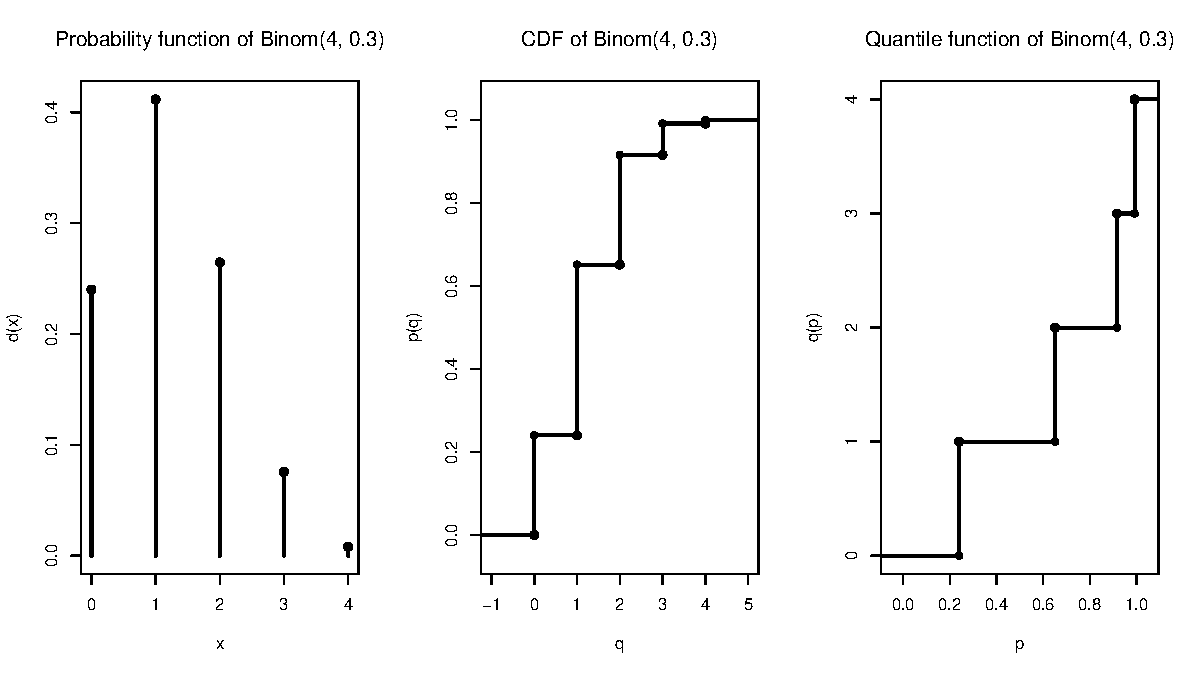
\includegraphics{distr-plotex4}
\end{figure}

\begin{figure}[p]
\begin{Schunk}
\begin{Sinput}
> B <- Binom(size = 4, prob = 0.3)
> plot(B, col="red", col.points = "green", main = TRUE, col.main="blue",
+      col.sub = "orange", sub = TRUE, cex.sub = 0.6, col.inner = "brown",
+      withSweave = TRUE)
\end{Sinput}
\end{Schunk}
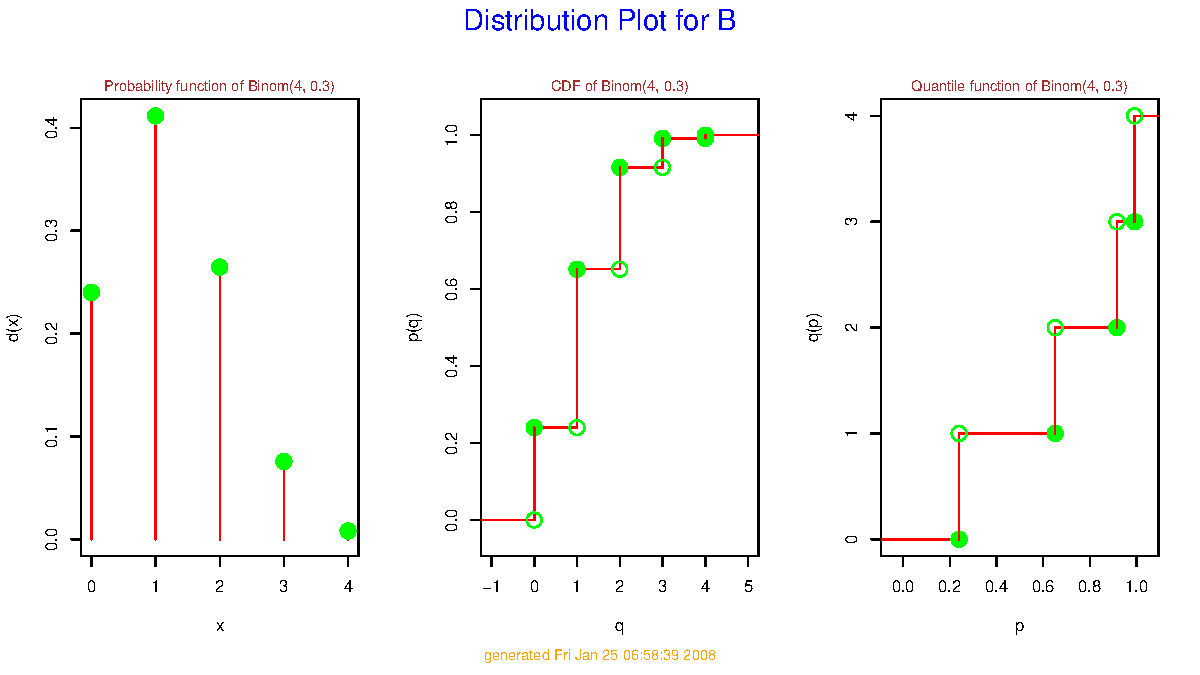
\includegraphics{distr-plotex5}
\end{figure}

\begin{figure}[p]
\begin{Schunk}
\begin{Sinput}
> plot(Nbinom(size = 4,prob = 0.3), cex.points = 1.2, pch.u = 20, pch.a = 10,
+      withSweave = TRUE)
\end{Sinput}
\end{Schunk}

\includegraphics{distr-plotex6}
\end{figure}

\begin{figure}[p]
\begin{Schunk}
\begin{Sinput}
> plot(Chisq(), log = "xy", ngrid = 100, withSweave = TRUE)
\end{Sinput}
\end{Schunk}
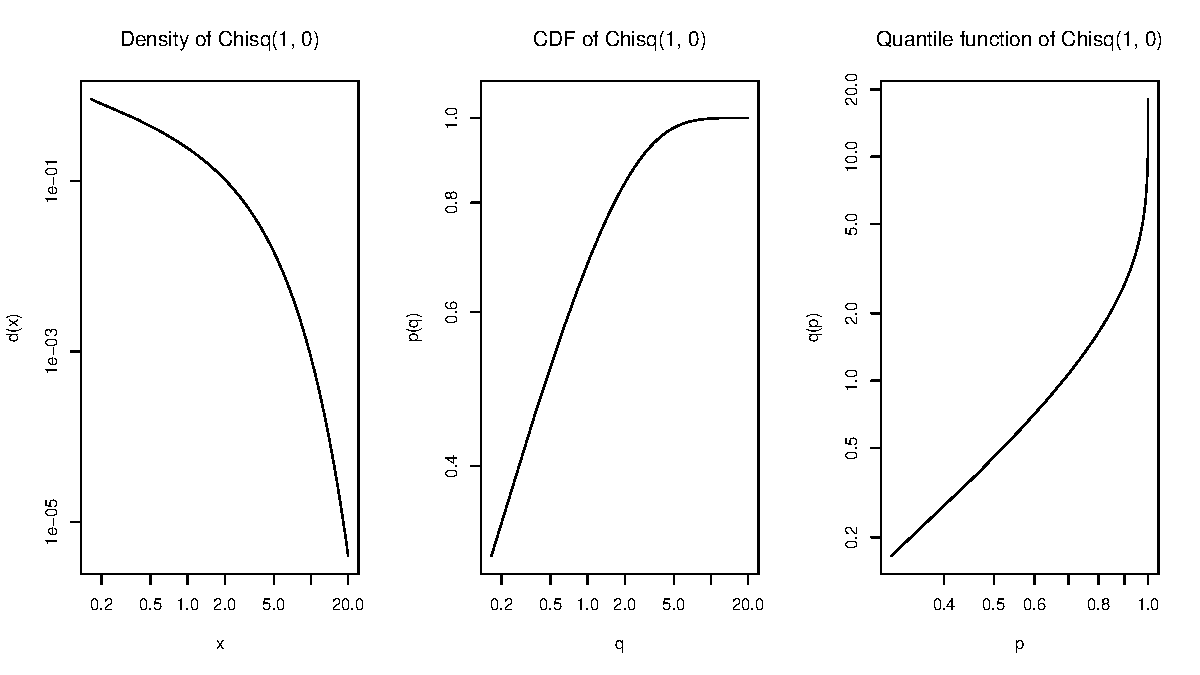
\includegraphics{distr-plotex7}
\end{figure}

\begin{figure}[p]
\begin{Schunk}
\begin{Sinput}
> plot(Norm(), lwd=3, col = "red", ngrid = 200, lty = 3, las = 2,
+      withSweave = TRUE)
\end{Sinput}
\end{Schunk}
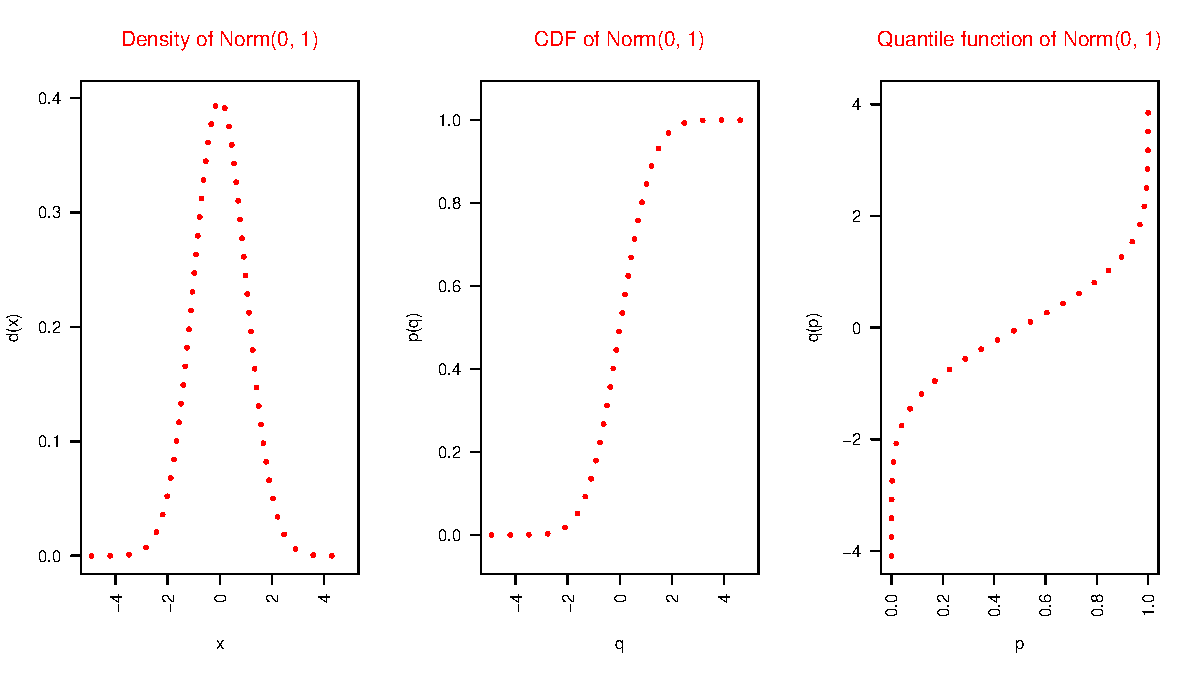
\includegraphics{distr-plotex8}
\end{figure}

\begin{figure}[p]
\begin{Schunk}
\begin{Sinput}
> plot(Norm(), main = "my Distribution: \%A",
+      inner = list(expression(paste(lambda, "-density of \%C(\%P)")), "CDF",
+                   "Pseudo-inverse with param's \%N"),
+      sub = "this plot was correctly generated on \%D",
+      cex.inner = 0.9, cex.sub = 0.8, withSweave = TRUE)
\end{Sinput}
\end{Schunk}
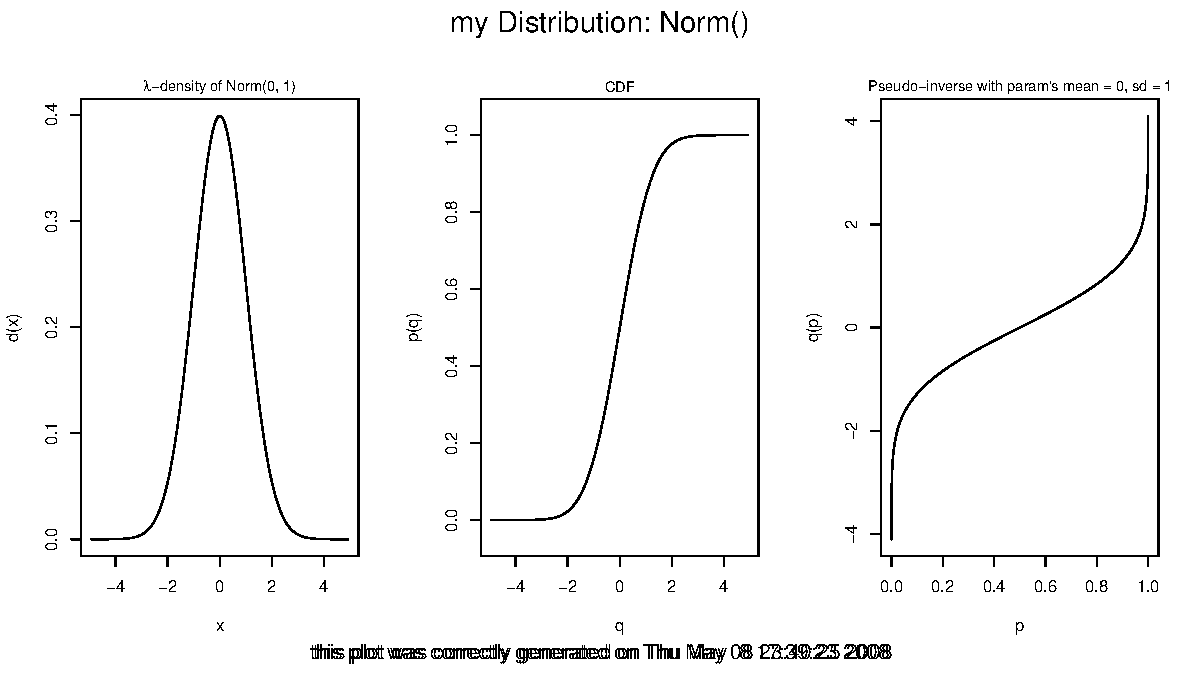
\includegraphics{distr-plotex9}
\end{figure}

\begin{figure}[p]
\begin{Schunk}
\begin{Sinput}
> Ch <- Chisq(); setgaps(Ch, exactq = 3)
> plot(Ch, cex = 1.2, pch.u = 20, pch.a = 10, col.points = "green", 
+      col.vert = "red", withSweave = TRUE)
\end{Sinput}
\end{Schunk}
\includegraphics{distr-plotex10}
\end{figure}

\par
For objects of  class \code{Dataclass} ---or of a corresponding subclass---
 \code{plot} plots the sample against the run index and in case  of  
 \code{ContSimulation} the contaminating variables are highlighted by a 
 different color. Additional arguments controlling
 the plot as in the default \code{plot} command may be passed, 
 confer \code{help("plot-methods",package="distrSim")}.
 \par
 For an object of class \code{Evaluation},
\code{plot} yields a boxplot of the results of the evaluation.
For an object of class \code{EvaluationList},
\code{plot} regroups the list according to the different columns/coordinates of 
the result of the evaluation; for each such coordinate, a boxplot is generated, 
containing possibly several procedures, and, if evaluated at a 
\code{Contsimulation}, the plots are also grouped into evaluations on ideal and
real data. As for the usual \code{boxplot} function you may pass additional 
``\code{plot}-type'' arguments to this particular \code{plot} method, confer 
\code{help("plot-methods",package="distrTEst")}. In particular, the 
\code{plot}-arguments \code{main} and \code{ylim}, however, may also be 
transmitted coordinatewise, i.e.; a vector of the same length as the dimension 
of the result {\tt resDim} (e.g.\ parameter dimension), respectively a 
{\tt 2 x resDim} matrix, or they may be transmitted globally, using the 
usual {\tt S} recycling rules.
%\newline??????1
\subsection[liesInSupport]{\code{liesInSupport}}
For all discrete distribution classes, we have methods \code{liesInSupport} to 
check whether a given vector/ a matrix of points lies in the support of the 
distribution.

\subsection[Simulation (in package distrSim)]%
{Simulation (in package \pkg{distrSim})}
%
From version 1.6 on, \code{simulation} is available in package  \pkg{distrSim}.

For the classes \code{Simulation} and \code{ContSimulation}, we normally will
not save the current values of the simulation, as they can easily be reproduced
knowing the values of the other slots of this class.
%
So when declaring a new object of either of the two classes, the slot 
\code{Data} will be empty (\code{NULL}).
To fill it with the simulated values, we have to apply the method 
\code{simulate} to the object. This has to be redone whenever another slot of 
the object is changed.
%
To guarantee reproducibility, we use the slot \code{seed}.\\
%
This slot is controlled and set through 
\href{mailto:pgilbert@bank-banque-canada.ca}{Paul Gilbert's} \pkg{setRNG} 
package.
By default, \code{seed} is set to \code{setRNG()}, which returns the current 
``state'' of the random number generator (RNG). So the user does not need to 
specify a value for \code{seed}, and nevertheless may reproduce his samples: 
He simply uses \code{simulate} to fill the \code{Data} slot.
If the user wants to, he may also set the \code{seed} explicitly via the 
replacement function \code{seed()}, but has to take care of the correct format 
himself, confer the documentation of \code{setRNG}. One easy way to fill 
the \code{Data} slot of a simulation \code{X} with ``new'' random numbers is
\begin{Schunk}
\begin{Sinput}
> have.distrSim <- suppressWarnings(require("distrSim"))
> if (have.distrSim)
+    {X <- Simulation()
+     seed(X) <- setRNG()
+     simulate(X)
+     print(Data(X)[1:10])
+    } else { 
+     cat("\n functionality not (yet) available; ")
+     cat("you have to install package \"distrSim\" first.\n")
+     }
\end{Sinput}
\begin{Soutput}
 [1]  0.8101505  1.1804566  0.2075169 -1.1013211  2.0973860 -1.7465246
 [7] -0.3640107 -1.4213738 -1.9721849  0.9657427
\end{Soutput}
\end{Schunk}
%
\subsection[Evaluate (in package distrTEst)]%
{Evaluate (in package \pkg{distrTEst})}\label{evaluate}
%
From version 1.6 on \code{evaluate} is available in  \pkg{distrTEst}.

In an object of class \code{Evaluation}  we store relevant information
about an evaluation of a statistical procedure (estimator/test/predictor)
on an object of class \code{Dataclass}, including the concrete results of
this evaluation. An object of class \code{Evaluation}  is generated by an 
application of method \code{evaluate} which takes as arguments an object of 
class  \code{Dataclass} and a procedure of type \code{function}. As an example, 
confer Example~\ref{simex}.
For data of class \code{Contsimulation}, the result takes a slightly different,
combining evalations on ideal and real data.
%
\subsection{Is-Relations}
%
By means of \code{setIs}, we have ``told'' {\sf R}  that a distribution object 
\code{obj} of class
\begin{itemize}
  \item  \code{"Unif"} with  $\code{Min} \doteq 0$ and  $\code{Max} \doteq 1$ 
   also is a Beta distribution with parameters \code{shape1 = 1, shape2 = 1}
  \item  \code{"Geom"} also is a negative Binomial distribution with parameters
         \code{size = 1, prob = prob(obj)}
  \item \code{"Cauchy"} with $\code{location} \doteq 0$ and 
         $\code{scale}\doteq 1$ also is a T distribution with parameters
         \code{df = 1, ncp = 0}
  \item \code{"Exp"} also is a Gamma distribution with parameters 
         \code{shape = 1, scale = 1/rate(obj)} and
         a Weibull  distribution with parameters 
         \code{shape = 1, scale = 1/rate(obj)}
  \item \code{"Chisq"} with non-centrality $\code{ncp}\doteq 0$ also is a 
        Gamma distribution with parameters \code{shape = df(obj)/2, scale = 2}
  \item \code{"DiscreteDistribution"}  (from version 1.9 on) with an equally 
         spaced support also is a \code{"LatticeDistribution"}
\end{itemize}
%
\subsection{Further methods}
%
When iterating/chaining mathematical operations on a univariate distribution,
generation process of random variables can become clumsy and slow.
To cope with this, we introduce a sort of ``Forget-my-past''-method 
\code{simplifyr} that replaces the  chain of mathematical operations in 
the \code{r}-method by drawing with replacement from a large 
sample ($10^{\tt RtoDPQ.e}$) of these.
%
\subsection[Functionals (in package distrEx)]%
{Functionals (in package \pkg{distrEx})}\label{Functionals}
%
\subsubsection{Expectation}
The most important contribution of package \pkg{distrEx} is a general 
expectation operator. In basic statistic courses, the expectation 
${\rm E}$ may come as ${\rm E}\,[X]$, ${\rm E}\,[f(X)]$, ${\rm E}\,[X|Y=y]$,
or ${\rm E}\,[f(X)|Y=y]$. Our operator (or in S4-language ``generic function'') 
\code{E} covers all of these situtations (or {\it signatures\/}).
\paragraph{default call}
The most frequent call will be \code{E(X)} where \code{X} is an (almost) 
arbitrary distribution object.
More precisely, if \code{X} is of a specific distribution class like 
\code{Pois}, it is evaluated exactly using analytic terms. Else if it is of 
class \code{DiscreteDistribution} we use a sum over the support of \code{X},
and if it is of class \code{AbscontDistribution} we use numerical 
integration\footnote{i.e., we first try (really(!): \code{try})
\code{integrate} and if this fails we use Gau{\ss}-Legendre integration 
according to \cite{NumR:92}, see also \code{?distrExIntegrate}}; if we only 
know that {\tt X} is of class \code{UnivariateDistribution} we use Monte-Carlo 
integration. This also is the default method in for class 
\code{MultivariateDistribution}, while for \code{DiscreteMVDistribution} we 
again use sums. For an object \code{Y} of a subclass of class 
union \code{AffLinDistribution}, we determine the expectation as 
\code{Y@a * E(Y@X0) + Y@b} and hence use analytic terms for \code{X0} if
available.

\paragraph{with a function as argument}
 we proceed just as without: if \code{X} is of class\linebreak[4]
 \code{DiscreteDistribution}, we use a sum over the support of \code{X},
and if \code{X} is of class\linebreak[4] \code{AbscontDistribution} we use numerical 
integration; else we use Monte-Carlo integration.
\paragraph{in addition: with a condition as argument} we simply use the 
corresponding \code{d} respective \code{r} slots with the additional 
argument \code{cond}.
\paragraph{exact evaluation}
is available for \code{X} of class \code{Beta} (for noncentrality $0$), 
\code{Binom}, \code{Cauchy}, \code{Chisq}, \code{Dirac}, \code{Exp}, \code{Fd}, 
\code{Gammad}, \code{Geom}, \code{Hyper}, \code{Logis}, \code{Lnorm}, 
\code{Nbinom}, \code{Norm}, \code{Pois}, \code{Td}, \code{Unif}, \code{Weibull}.
\paragraph{examples} $ \mbox{ }$\newline
\begin{Schunk}
\begin{Sinput}
> have.distrEx <- suppressWarnings(require("distrEx"))
> if (have.distrEx) 
+     {D4 <- LMCondDistribution(theta = 1)
+      D4  # corresponds to Norm(cond, 1)
+      N <- Norm(mean = 2)
+ 
+      print(E(D4, cond = 1))
+      print(E(D4, cond = 1, useApply = FALSE))
+      print(E(as(D4, "UnivariateCondDistribution"), cond = 1))
+      print(E(as(D4, "UnivariateCondDistribution"), cond = 1,
+        useApply = FALSE))
+      print(E(D4, function(x){x^2}, cond = 2))
+      print(E(D4, function(x){x^2}, cond = 2, useApply = FALSE))
+      print(E(N, function(x){x^2}))
+      print(E(as(N, "UnivariateDistribution"), function(x){x^2},
+        useApply = FALSE)) # crude Monte-Carlo
+      print(E(D4, function(x, cond){cond*x^2}, cond = 2,
+        withCond = TRUE))
+      print(E(D4, function(x, cond){cond*x^2}, cond = 2,
+        withCond = TRUE, useApply = FALSE))
+      print(E(N, function(x){2*x^2}))
+      print(E(as(N, "UnivariateDistribution"), function(x){2*x^2},
+        useApply = FALSE)) # crude Monte-Carlo
+      Y <- 5 * Binom(4, .25) - 3
+      print(Y); print(E(Y))  
+     } else {
+     cat("\n functionality not (yet) available; ")
+     cat("you have to install package \"distrEx\" first.\n")
+     }